%%%%%%%%%%%%%%%%%%%%%%%%%%%%%%%%%%%%%%%%%%%%%%%%%%%%%%%%%%%%%%%%%%%%%%%%%%%%%
%% Matematika Dasar: Pengantar Masuk ke Alam Pikir Kecerdasan Buatan       %%                                  
%% Penyusun: Sandy Herho (sandyherho.github.io) dan Dasapta Erwin Irawan   %%
%% License: CC0.v1                                                         %%
%%%%%%%%%%%%%%%%%%%%%%%%%%%%%%%%%%%%%%%%%%%%%%%%%%%%%%%%%%%%%%%%%%%%%%%%%%%%%

\documentclass[b5paper,11pt]{book}
\usepackage[T1]{fontenc}
\usepackage[utf8]{inputenc}
\usepackage{lmodern}
\usepackage{hyperref}
\usepackage{hyperref}
\usepackage{graphicx}
\usepackage{breqn}
\usepackage[bahasa]{babel}
\usepackage{float}
\usepackage{fancyvrb}
\usepackage{longtable}
\usepackage{tabularx}
\usepackage{xcolor}
\usepackage[most]{tcolorbox}
\usepackage{mathtools}
\usepackage{xfrac}  
\usepackage{optidef}
\usepackage{enumitem}
\setcounter{secnumdepth}{0}
\DeclarePairedDelimiter{\norm}{\lVert}{\rVert}
\DeclareMathOperator*{\minimize}{min}

% R
\lstset{frame=tb,
language=R,
keywordstyle=\color{blue},
alsoletter={.}
}

%Jupyter

\definecolor{white}{rgb}{1,1,1}
\definecolor{mygreen}{rgb}{0,0.4,0}
\definecolor{light_gray}{rgb}{0.97,0.97,0.97}
\definecolor{mykey}{rgb}{0.117,0.403,0.713}

\tcbuselibrary{listings}
\newlength\inwd
\setlength\inwd{1.3cm}

\newcounter{ipythcntr}
\renewcommand{\theipythcntr}{\texttt{[\arabic{ipythcntr}]}}

\newtcblisting{pyin}[1][]{%
  sharp corners,
  enlarge left by=\inwd,
  width=\linewidth-\inwd,
  enhanced,
  boxrule=0pt,
  colback=light_gray,
  listing only,
  top=0pt,
  bottom=0pt,
  overlay={
    \node[
      anchor=north east,
      text width=\inwd,
      font=\footnotesize\ttfamily\color{mykey},
      inner ysep=2mm,
      inner xsep=0pt,
      outer sep=0pt
      ] 
      at (frame.north west)
      {\refstepcounter{ipythcntr}\label{#1}In \theipythcntr:};
  }
  listing engine=listing,
  listing options={
    aboveskip=1pt,
    belowskip=1pt,
    basicstyle=\footnotesize\ttfamily,
    language=Python,
    keywordstyle=\color{mykey},
    showstringspaces=false,
    stringstyle=\color{mygreen}
  },
}
\newtcblisting{pyprint}{
  sharp corners,
  enlarge left by=\inwd,
  width=\linewidth-\inwd,
  enhanced,
  boxrule=0pt,
  colback=white,
  listing only,
  top=0pt,
  bottom=0pt,
  overlay={
    \node[
      anchor=north east,
      text width=\inwd,
      font=\footnotesize\ttfamily\color{mykey},
      inner ysep=2mm,
      inner xsep=0pt,
      outer sep=0pt
      ] 
      at (frame.north west)
      {};
  }
  listing engine=listing,
  listing options={
      aboveskip=1pt,
      belowskip=1pt,
      basicstyle=\footnotesize\ttfamily,
      language=Python,
      keywordstyle=\color{mykey},
      showstringspaces=false,
      stringstyle=\color{mygreen}
    },
}
\newtcblisting{pyout}[1][\theipythcntr]{
  sharp corners,
  enlarge left by=\inwd,
  width=\linewidth-\inwd,
  enhanced,
  boxrule=0pt,
  colback=white,
  listing only,
  top=0pt,
  bottom=0pt,
  overlay={
    \node[
      anchor=north east,
      text width=\inwd,
      font=\footnotesize\ttfamily\color{mykey},
      inner ysep=2mm,
      inner xsep=0pt,
      outer sep=0pt
      ] 
      at (frame.north west)
      {\setcounter{ipythcntr}{\value{ipythcntr}}Out#1:};
  }
  listing engine=listing,
  listing options={
      aboveskip=1pt,
      belowskip=1pt,
      basicstyle=\footnotesize\ttfamily,
      language=Python,
      keywordstyle=\color{mykey},
      showstringspaces=false,
      stringstyle=\color{mygreen}
    },
}
%Jupyter

% listing
\usepackage{listings}
\usepackage{color}
\usepackage{float}
\usepackage{verbatim}
\usepackage{alltt}
\usepackage{caption}
\usepackage{gensymb}
\usepackage[super]{nth}



%warna baru
\definecolor{codegreen}{rgb}{0,0.6,0}
\definecolor{codegray}{rgb}{0.5,0.5,0.5}
\definecolor{codepurple}{rgb}{0.58,0,0.82}
\definecolor{backcolour}{rgb}{0.95,0.95,0.92}

%code listing dinamakan "mystyle"
\lstdefinestyle{mystyle}{
  backgroundcolor=\color{backcolour},   commentstyle=\color{codegreen},
  keywordstyle=\color{magenta},
  numberstyle=\tiny\color{codegray},
  stringstyle=\color{codepurple},
  basicstyle=\footnotesize,
  breakatwhitespace=false,         
  breaklines=true,                 
  captionpos=b,                    
  keepspaces=true,                 
  numbers=left,                    
  numbersep=5pt,                  
  showspaces=false,                
  showstringspaces=false,
  showtabs=false,                  
  tabsize=2
}

%"mystyle" code listing set
\lstset{style=mystyle}
%listing

%%%%%%%%%%%%%%%%%%%%%%%%%%%%%%%%%%%%%%%%%%%%%%%%%%%%%%%%%%%%%%%%%%%%%%%%%%%%%%%%
% halaman dedikasi                                                             % 
%%%%%%%%%%%%%%%%%%%%%%%%%%%%%%%%%%%%%%%%%%%%%%%%%%%%%%%%%%%%%%%%%%%%%%%%%%%%%%%%
\newenvironment{dedication}
{
   \cleardoublepage
   \thispagestyle{empty}
   \vspace*{\stretch{1}}
   \hfill\begin{minipage}[t]{0.66\textwidth}
   \raggedright
}
{
   \end{minipage}
   \vspace*{\stretch{3}}
   \clearpage
}

%%%%%%%%%%%%%%%%%%%%%%%%%%%%%%%%%%%%%%%%%%%%%%%%

%%%%%%%%%%%%%%%%%%%%%%%%%%%%%%%%%%%%%%%%%%%%%%%%
\makeatletter
\renewcommand{\@chapapp}{}
\newenvironment{chapquote}[2][2em]
  {\setlength{\@tempdima}{#1}%
   \def\chapquote@author{#2}%
   \parshape 1 \@tempdima \dimexpr\textwidth-2\@tempdima\relax%
   \itshape}
  {\par\normalfont\hfill--\ \chapquote@author\hspace*{\@tempdima}\par\bigskip}
\makeatother

%%%%%%%%%%%%%%%%%%%%%%%%%%%%%%%%%%%%%%%%%%%%%%%%%%%%%%%%%%%%%%%%%%%%%%%%%%%%%%%%%%%%%%%%%%%%%%%%%%
% Halaman awal dalam buku yang memuat hal - hal seperti:Judul Buku, sub-judul, dan nama penyusun.%
%%%%%%%%%%%%%%%%%%%%%%%%%%%%%%%%%%%%%%%%%%%%%%%%%%%%%%%%%%%%%%%%%%%%%%%%%%%%%%%%%%%%%%%%%%%%%%%%%%

% Judul Buku dan Sub-Judul
\title{\mbox{\textbf{\huge Matematika Dasar}} \\ \\
\small Pengantar Menuju Analisis Data}
% penyusun
\author{\textsc{Sandy Hardian Susanto Herho}\thanks{ \href{mailto:sandyherho@protonmail.ch}{sandyherho@protonmail.ch} }}


\begin{document}

\frontmatter
\maketitle
%%%%%%%%%%%%%%%%%%%%%%%%%%%%%%%%%%%%%%%%%%%%%%%%%%%%%%%%%%%%%%%
% Dedikasi Buku %
%%%%%%%%%%%%%%%%%%%%%%%%%%%%%%%%%%%%%%%%%%%%%%%%%%%%%%%%%%%%%%%
\begin{dedication}
Untuk publik sains terbuka Indonesia.\\
\end{dedication}

%%%%%%%%%%%%%%%%%%%%%%%%%%%%%%%%%%%%%%%%%%%%%%%%%%%%%%%%%%%%%%%%%%%%%%%%
% DAFTAR Isi                                                           %
%%%%%%%%%%%%%%%%%%%%%%%%%%%%%%%%%%%%%%%%%%%%%%%%%%%%%%%%%%%%%%%%%%%%%%%%

\chapter*{Kata Pengantar}

Keilmuan analisis data menjadi primadona dalam perbincangan global di satu dekade terakhir. Hal ini ditandai dengan semakin terintegrasinya kehidupan umat manusia dengan teknologi yang berbuntut dengan lahirnya kumpulan data raksasa (\textit{big data}) yang dapat kemudian dijadikan bahan bagi pemelajaran algoritma kecerdasan buatan untuk menghasilkan produk yang diharapkan dapat beradaptasi dengan kebutuhan pengguna. 

Kecerdasan buatan di dalam beberapa waktu terakhir ini juga menelurkan perkembangan cukup pesat. Hal ini ditandai dengan terciptanya mobil swakemudi (\textit{self-driving car}), diagnosa medis mutakhir, sistem kecerdasan yang dapat mengalahkan manusia dalam permainan catur dan GO, dll.

Progres di dalam penelitian dan pengembangan kecerdasan buatan tampak menjanjikan. Bukan tidak mungkin dalam beberapa dekade mendatang kita dapat membangun sistem kecerdasan buatan umum (\textit{Artificial General Intelligence}) yang dapat menggantikan profesi manusia. Namun untuk mencapai hal tersebut diperlukan kerja keras dan kecerdasan dari para peneliti dan pengembang untuk menemukan dan mengeksekusi algoritma kecerdasan buatan hingga mencapai tahap siap untuk diproduksi secara massal. Mimpi ini tentu tidaklah mudah untuk dicapai karena untuk berkontribusi di dalam penelitian dan pengembangan algoritma kecerdasan buatan diperlukan dasar kemampuan matematis dan pemrograman yang cukup kuat.

Melalui catatan singkat ini penyusun hendak mengajak pembaca untuk berkenalan dengan konsep - konsep matematika yang diperlukan sebagai fondasi untuk memahami dan mengimplementasikan algoritma - algoritma yang digunakan di dalam analisis data melalui bahasa pemrograman Python dan R (penyusun mengharapkan familiaritas pembaca terhadap konsep - konsep kedua bahasa pemrograman tersebut sebelum mempelajari buku ini). 

Catatan ini sendiri didesain sebagai jembatan kesenjangan pengetahuan di dunia industri dan dunia akademik terkait konsep - konsep dasar matematika yang dibutuhkan bagi para analis data junior, pengembang piranti lunak, mahasiswi/a dari jurusan non-eksakta, dan kaum awam guna berkontribusi di dalam pengembangan kecerdasan buatan melalui analisis data.

Buku ini akan membahas tiga konsep matematika utama yang menjadi fondasi algoritma kecerdasan buatan jaringan saraf tiruan (\textit{neural networks}), yakni aljabar linier, kalkulus peubah banyak, dan teori probabilitas. 

Selain konsep - konsep matematika, pembaca juga akan disuguhkan laboratorium pemrograman kecil pada setiap bab-nya dan latihan pemahaman konsep di bagian akhir buku. Pembaca diharapkan dapat memahami dan mengimplementasikan konsep - konsep matematika yang diterangkan di sini pada bidang keilmuannya masing - masing ketika selesai mempelajari catatan ini. 

Catatan ini juga bersifat sumber terbuka, karena dituliskan dengan menggunakan \LaTeX{} dan berlisensi milik publik (\textit{copy-left}), sehingga para pembaca dapat menyalin dan mengubahnya, bahkan untuk kepentingan komersil sekalipun, secara cuma - cuma di \url{https://github.com/sandyherho/buku-mat-andat}. 

Akhir kata, semoga catatan singkat dapat membantu dan saya menanti dengan tangan terbuka kolaborasi pembelajaran berbasis kode terbuka di laman GitHub penyusun.  

\mbox{}\\
%\mbox{}\\
\noindent Penyusun \\\\

\tableofcontents
%\listoffigures
%\listoftables

%%%%%%%%%%%%%%%%
% ISI %
%%%%%%%%%%%%%%%%
\mainmatter
\chapter{Aljabar Linier}

\section{Skalar, vektor, matriks, dan tensor}
\subsection{Definisi skalar, vektor, dan matriks}
Berikut ini merupakan definisi praktis dari sudut pandang keilmuan kecerdasan buatan untuk ketiga objek utama di dalam keilmuan aljabar linier ini:
\begin{itemize}
    \item Skalar ($x$): nilai tunggal tanpa dimensi. Formulasi umumnya adalah:
    \begin{equation}\label{eqn:eqn1}
        X
    \end{equation}
    
    Contoh:
    \begin{equation*}
        x = 12
    \end{equation*}
    \item Vektor ($\mathbf{x}$): himpunan bilangan (\textit{array}) berdimensi tunggal yang dapat berupa kolom ataupun baris dan dapat diidentifikasi melalui baris dan kolom.  Formulasi umumnya adalah: 
    \begin{equation}\label{eqn:eqn2}
        \begin{bmatrix}X_{0} & X_{1} & \cdots &  X_{n}\end{bmatrix} \text{ atau } \begin{bmatrix}X_{0} \\ X_{1} \\ \vdots \\ X_{n}\end{bmatrix}
    \end{equation}
    
    Contoh:
    \begin{equation*}
        \mathbf{x} = \begin{bmatrix}1 & 2 & 3\end{bmatrix} \text{ atau } \mathbf{x} = \begin{bmatrix}1 \\ 2 \\ 3\end{bmatrix}
    \end{equation*}
    \item Matriks ($\mathbf{X}$): \textit{Array} berdimensi dua\footnote{Dimensi umumnya didefinisikan dalam format baris, kolom. Matriks merupakan \textit{array} berdimensi dua karena mempunyai baris dan kolom, sementara vektor berdimensi tunggal karena hanya mempunyai baris atau kolom.}, di mana setiap elemennya dapat diakses melalui indeks baris dan kolom\footnote{Pengindeksan yang penyusun gunakan pada catatan ini berbeda dengan kebanyakan pengindeksan yang dijabarkan pada buku teks aljabar linier karena dalam kontek kecerdasan buatan yang lebih dekat pada dunia ilmu komputer, umumnya digunakan pengindeksan yang dimulai dari nol.}. Formulasi umumnya adalah:
    \begin{equation}\label{eqn:eqn3}
        \textbf{X} = \begin{bmatrix}X_{0,0} & X_{0,1} & \cdots & X_{0,n}\\X_{1,0} & X_{1,1} & \cdots & X_{1,n}\\ \cdots & \cdots & \cdots & \cdots \\X_{m,0} & X_{m,1} & \cdots & X_{m,n} \end{bmatrix}
    \end{equation}
    
    Contoh:
    \begin{equation*}
        \textbf{X} = \begin{bmatrix}1 & 2 & 3\\4 & 5 & 6\end{bmatrix}
    \end{equation*}
\end{itemize}

\subsection{Operasi antar matriks}
Operasi matriks seperti penjumlahan, pengurangan, dan perkalian sangat lazim dijumpai di dalam algoritma pemelajaran mesin.
\subsubsection{Penjumlahan dan Pengurangan Matriks}
Penjumlahan atau pengurangan matriks merupakan operasi penjumlahan atau pengurangan antar elemen dengan indeks yang sama pada kedua matriks, oleh karena itu prasyarat utamanya adalah kedua matriks yang hendak dijumlahkan harus mempunyai dimensi yang sama. Penjumlahan atau pengurangan antar matriks $\mathbf{A}$ dan $\mathbf{B}$ akan menghasilkan matriks $\mathbf{C}$ dengan dimensi yang sama. Berikut adalah formulasi umum operasi penjumlahan atau pengurangan antar matriks tersebut:
\begin{dmath}\label{eqn:eqn4}
    \textbf{A} \pm \textbf{B} = \begin{bmatrix}a_{0,0} & a_{0,1} & \cdots & a_{0,n}\\ a_{1,0} & a_{1,1} & \cdots & a_{1,n} \\ \vdots & \vdots & \ddots & \vdots \\ a_{m,0} & a_{m,1} & \cdots & a_{m,n}\end{bmatrix} + \begin{bmatrix}b_{0,0} & b_{0,1} & \cdots & b_{0,n}\\ b_{1,0} & b_{1,1} & \cdots & b_{1,n} \\ \vdots & \vdots & \ddots & \vdots \\ b_{m,0} & b_{m,1} & \cdots & b_{m,n}\end{bmatrix} = \begin{bmatrix}a_{0,0} \pm b_{0,0} & a_{0,1} \pm b_{0,1} & \cdots & a_{0,n} \pm b_{0,n}\\ a_{1,0} \pm b_{1,0} & a_{1,1} \pm b_{1,1} & \cdots & a_{1,n} \pm b_{1,n} \\ \vdots & \vdots & \ddots & \vdots \\ a_{m,0} \pm b_{m,0} & a_{m,1} \pm b_{m,1} & \cdots & a_{m,n} \pm b_{m,n}\end{bmatrix}
\end{dmath}

Contoh:
\begin{equation*}
    \textbf{A} + \textbf{B} = \begin{bmatrix}1 & 2 & 3 \\ 4 & 5 & 6\end{bmatrix} + \begin{bmatrix}2 & 1 & 4\\ 1 & 1 & 2\end{bmatrix} = \begin{bmatrix}3 & 3 & 7 \\ 5 & 6 & 8 \end{bmatrix}
\end{equation*}

\begin{equation*}
    \mathbf{A} - \mathbf{B} = \begin{bmatrix}1 & 2 & 3 \\ 4 & 5 & 6\end{bmatrix} - \begin{bmatrix}2 & 1 & 4\\ 1 & 1 & 2\end{bmatrix} = \begin{bmatrix}-1 & 1 & -1 \\ 3 & 4 & 4\end{bmatrix}
\end{equation*}

\subsubsection{Perkalian matriks}
Perkalian antar matriks $\mathbf{A}$ dan $\mathbf{B}$ akan menghasilkan matriks baru, yakni $\mathbf{C}$. Untuk melakukan operasi perkalian ini, matriks $\mathbf{A}$ harus mempunyai jumlah kolom yang sama dengan jumlah baris pada matriks $\mathbf{B}$. Berikut adalah formulasi umum perkalian antar kedua matriks:

\begin{dmath*}
    \begin{bmatrix}a_{0,0} & a_{0,1}\\ a_{1,0} & a_{1,1}\end{bmatrix} * \begin{bmatrix} b_{0,0} & b_{0,1}\\ b_{1,0} & b_{1,1}\end{bmatrix} =
    \begin{bmatrix}a_{0,0}b_{0,0} + a_{0,1}b_{1,0} & a_{0,0}b_{0,1} + a_{0,1}b_{1,1}\\a_{0,1}b_{0,0} + a_{1,1}b_{1,0} & a_{1,0}b_{0,1} + a_{1,1}b_{1,1} \end{bmatrix} =
    \begin{bmatrix} 
    c_{0,0} & c_{0,1}\\
    c_{1,0} & c_{1,1}
    \end{bmatrix}
\end{dmath*}
Atau secara umum dapat diformulasikan seperti pada persamaan \ref{eqn:eqn5} berikut ini:
\begin{dmath}\label{eqn:eqn5}
    \mathbf{C}_{i,j} = \Sigma_{k} \mathbf{A}_{i,k}\mathbf{B}_{j,k}
\end{dmath}
Perkalian matriks juga dapat terjadi pada matriks yang mempunyai dimensi yang berbeda, asalkan matriks pertama mempunyai kolom yang sama dengan jumlah baris pada matriks kedua,seperti pada contoh berikut ini:
\begin{dmath*}
    \begin{bmatrix}1 & 2\\3 & 4\\5 & 6\end{bmatrix} * \begin{bmatrix}1 & 3 & 5\\2 & 4 & 6\end{bmatrix} = \begin{bmatrix}1(1) + 2(2) & 1(3) + 2(4) & 1(5) + 2(6)\\3(1) + 4(2) & 3(3) + 4(4) & 3(5) + 4(6)\\ 5(1) + 6(2) & 5(3) + 6(4) & 5(5) + 6(6)\end{bmatrix} = \begin{bmatrix}5 & 11 & 17\\11 & 25 & 39\\17 & 39 & 61\end{bmatrix}
\end{dmath*}
Terdapat dua buah karakteristik utama dari perkalian matriks, yakni:
\begin{enumerate}
    \item Distributif: 
        \begin{equation} \label{eqn:eqn6}
            \mathbf{A}\left(\mathbf{B} + \mathbf{C}\right) = \mathbf{A}\mathbf{B} + \mathbf{A}\mathbf{C}
        \end{equation}
    \item Asosiatif: 
        \begin{equation}\label{eqn:eqn7}
            \mathbf{A}\left(\mathbf{B}\mathbf{C}\right) = \left(\mathbf{A}\mathbf{B}\right)\mathbf{C}
        \end{equation}
\end{enumerate}
\subsection{Transpos}
Transpos merupakan operasi menukar indeks matriks pada diagonal utamanya. Dengan kata lain, transpos menukar indeks baris menjadi indeks kolom, dan sebaliknya.

Berikut ini adalah contohnya:
\[
    \begin{bmatrix}a_{0,0} & a_{0,1} & a_{0,2}\\ a_{1,0} & a_{1,1} & a_{1,2}\\a_{2,0} & a_{2,1} & a_{2,2}\end{bmatrix}^{T} = \begin{bmatrix}a_{0,0} & a_{1,0} & a_{2,0} \\ a_{0,1} & a_{1,1} & a_{2,1} \\ a_{0,2} & a_{1,2} & a_{2,2}\end{bmatrix}
\]

\[
\begin{bmatrix}1 & 2 & 3\\4 & 5 & 6\\7 & 8 & 9\end{bmatrix} = \begin{bmatrix} 1 & 4 & 7 \\ 2 & 5 & 8\\ 3 & 6 & 9\end{bmatrix}
\]

Berikut ini merupakan contoh operasi transpos pada matriks dengan dimensi baris dan kolom yang berbeda:

\[
\begin{bmatrix}1 & 2 \\ 3 & 4 \\ 5 & 6\end{bmatrix}^{T} = \begin{bmatrix}1 & 3 & 5\\2 & 4 & 6\end{bmatrix}
\]

Kita juga dapat melakukan operasi transpos pada vektor. Operasi transpos vektor ini lah yang sering digunakan dalam pemrosesan dan pembersihan data sebelum dijadikan input algoritma pemelajaran mesin:

\[
\begin{bmatrix} 1 & 2 & 3\end{bmatrix}^{T} = \begin{bmatrix} 1\\2\\3\end{bmatrix}
\]


\subsection{Tensor}
Terkadang di dalam era data raksasa seperti saat ini, kita harus berurusan dengan data yang mempunyai sumbu dimensi lebih dari dua. Data dengan sumbu dimensi banyak inilah yang dinamakan tensor (vektor dan matriks juga termasuk ke dalam tensor dimensi satu dan dua, lihat Gambar \ref{fig:fig1}) . Operasi dan fitur yang ditawarkan oleh tensor sama seperti yang telah kita ketahui pada vektor dan matriks, hanya saja berbeda pada dimensi saja, dan hal ini dapat dengan mudah diatasi oleh kemajuan fasilitas komputasi numerik saat ini.

\begin{figure}[H]
    \centering
    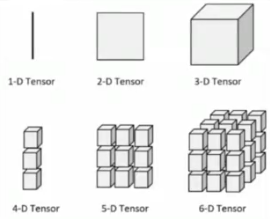
\includegraphics[width=0.5\textwidth]{gambar/gmb1.png}
    \caption{Ilustrasi tensor.}
    \label{fig:fig1}
\end{figure}

\section{Laboratorium 1: skalar, vektor, matriks, dan tensor}
Pada bagian ini, kita akan mencoba untuk mengimplementasikan konsep - konsep yang telah kita pelajari di lingkungan komputasi Python, khususnya dengan menggunakan pustaka numerik NumPy. Untuk itu, kita harus memastikan bahwa lingkungan yang kita gunakan telah sesuai, jalankan perintah berikut ini di Jupyter Notebook kalian masing - masing:

\subsection{Memulai sesi NumPy}
\begin{pyin}
import sys
import numpy as np

print("Python: {}".format(sys.version))
print("NumPy: {}".format(np.__version__))
\end{pyin}

\begin{pyin}
Python: 3.8.3 (default, May 19 2020, 18:47:26) 
[GCC 7.3.0]
NumPy: 1.18.1
\end{pyin}

Kita dapat mendefinisikan skalar (yang mana merupakan nilai bilangan tunggal) dengan menggunakan operator \verb|=| untuk penugasan ke suatu variabel tertentu:

\begin{pyin}
# penugasan skalar
x = 128
x
\end{pyin}

\begin{pyout}
128
\end{pyout}

Dengan NumPy, kita dapat mendefinisikan vektor dengan menggunakan fungsi \verb|array()|:
\begin{pyin}
# penugasan vektor
x = np.array((1,2,8))
x
\end{pyin}
\begin{pyout}
array([1, 2, 8])
\end{pyout}

\textit{Array} mempunyai beberapa atribut yang dapat memberitahu kita tentang informasi terkait dimensi dan ukuran suatu vektor:

\begin{pyin}
print("Dimensi vektor: {}".format(x.shape))
print("Ukuran vektor: {}".format(x.size))
\end{pyin}
\begin{pyout}
Dimensi vektor: (3,)
Ukuran vektor: 3
\end{pyout}

Untuk mendefinisikan matriks, kita dapat menggunakan fungsi \verb|matrix()| di pustaka NumPy. Guna memisahkan baris antar matriksnya, kita dapat menggunakan tanda \verb|[]| dan koma:

\begin{pyin}
X = np.matrix([[1,2,8],[2,2,0],[3,2,0]])
X
\end{pyin}
\begin{pyout}
matrix([[1, 2, 8],
        [2, 2, 0],
        [3, 2, 0]])        
\end{pyout}


Untuk mengetahui dimensi dan ukuran matriks $X$, kita dapat menggunakan perintah yang sama:

\begin{pyin}
print('Dimensi matriks: {}'.format(X.shape))
print('Ukuran matriks: {}'.format(X.size))
\end{pyin}
\begin{pyout}
Dimensi matriks: (3, 3)
Ukuran matriks: 9
\end{pyout}
NumPy memudahkan kita untuk mendefinisikan matriks secara cepat, misalkan pada kasus ini kita hendak mendefinisikan matriks identitas $3 \times 3$, kita tinggal menggunakan fungsi \verb|ones()|:
\begin{pyin}
X = np.ones((3,3))
X
\end{pyin}
\begin{pyout}
array([[1., 1., 1.],
       [1., 1., 1.],
       [1., 1., 1.]])
\end{pyout}

\begin{pyin}
print('Dimensi matriks: {}'.format(X.shape))
print('Ukuran matriks: {}'.format(X.size))
\end{pyin}

\begin{pyout}
Dimensi matriks: (3, 3)
Ukuran matriks: 9
\end{pyout}

Sebagai manusia yang hidup di ruang tiga dimensi, tentu kita akan sangat kesulitan ketika memvisualisasikan tensor berdimensi banyak, namun NumPy mempermudah kita untuk melakukan pendefinisian ini dengan menggunakan satu baris perintah:
\begin{pyin}
X = np.ones((3,3,3))
X
\end{pyin}
\begin{pyout}
array([[[1., 1., 1.],
        [1., 1., 1.],
        [1., 1., 1.]],

       [[1., 1., 1.],
        [1., 1., 1.],
        [1., 1., 1.]],

       [[1., 1., 1.],
        [1., 1., 1.],
        [1., 1., 1.]]])
\end{pyout}
\begin{pyin}
print("Dimensi tensor: {}".format(x.shape))
print("Ukuran tensor: {}".format(x.size))
\end{pyin}
\begin{pyout}
Dimensi tensor: (3,)
Ukuran tensor: 3
\end{pyout}
\subsection{Pengindeksan}
Bagian ini mencoba untuk memfamiliarkan konvensi pengindeksan NumPy.
\begin{pyin}
A = np.ones((5,5), dtype = np.int)
print(A)
\end{pyin}

\begin{pyout}
\%[[1 1 1 1 1]
 [1 1 1 1 1]
 [1 1 1 1 1]
 [1 1 1 1 1]
 [1 1 1 1 1]]
\end{pyout}
\begin{pyin}
# pengindeksan dimulai dari 0
A[0,1] = 2
print(A)
\end{pyin}
\begin{pyout}
\%[[1 2 1 1 1]
 [1 1 1 1 1]
 [1 1 1 1 1]
 [1 1 1 1 1]
 [1 1 1 1 1]]
\end{pyout}
\begin{pyin}
# Penting untuk dicatat jika NumPy melakukan pengindeksan dengan konvensi baris, kolom 
# Kita dapat melakukan penugasan seluruh baris atau kolom dengan menggunakan operator : 
A[:,0] = 3
print(A)
\end{pyin}
\begin{pyout}
\%[[3 2 1 1 1]
 [3 1 1 1 1]
 [3 1 1 1 1]
 [3 1 1 1 1]
 [3 1 1 1 1]]
\end{pyout}
\begin{pyin}
# Hal ini berlaku juga untuk Tensor berdimensi banyak 
A = np.ones((5,5,5), dtype = np.int)

# Berikut ini contohnya
A[:,0,0] = 128
print(A)
\end{pyin}
\begin{pyout}
\%[[[128   1   1   1   1]
  [  1   1   1   1   1]
  [  1   1   1   1   1]
  [  1   1   1   1   1]
  [  1   1   1   1   1]]

 [[128   1   1   1   1]
  [  1   1   1   1   1]
  [  1   1   1   1   1]
  [  1   1   1   1   1]
  [  1   1   1   1   1]]

 [[128   1   1   1   1]
  [  1   1   1   1   1]
  [  1   1   1   1   1]
  [  1   1   1   1   1]
  [  1   1   1   1   1]]

 [[128   1   1   1   1]
  [  1   1   1   1   1]
  [  1   1   1   1   1]
  [  1   1   1   1   1]
  [  1   1   1   1   1]]

 [[128   1   1   1   1]
  [  1   1   1   1   1]
  [  1   1   1   1   1]
  [  1   1   1   1   1]
  [  1   1   1   1   1]]]
\end{pyout}
\subsection{Operasi antar matriks}
Bagian ini merupakan demo operasi penjumlahan, pengurangan, dan perkalian matriks.
\begin{pyin}
A = np.matrix([[1,2],[3,4]])
B = np.ones((2,2), dtype = np.int)
\end{pyin}
\begin{pyin}
print(A)
\end{pyin}
\begin{pyout}
\%[[1 2]
 [3 4]]
\end{pyout}
\begin{pyin}
print(B)
\end{pyin}
\begin{pyout}
\%[[1 1]
 [1 1]]
\end{pyout}
\begin{pyin}
# Penjumlahan antar elemen
C = A + B
print(C)
\end{pyin}
\begin{pyout}
\%[[2 3]
 [4 5]]
\end{pyout}
\begin{pyin}
# Pengurangan antar elemen
C = A - B
print(C)
\end{pyin}
\begin{pyout}
\%[[0 1]
 [2 3]]
\end{pyout}
\begin{pyin}
# Perkalian matriks
C = A*B
print(C)
\end{pyin}
\begin{pyout}
\%[[3 3]
 [7 7]]
\end{pyout}
\subsection{Transpos matriks}
Seperti yang telah kita pelajari, transpos digunakan untuk menukar elemen antar baris dan kolom pada suatu array. NumPy memudahkan kita untuk melakukan operasi transpos matriks secara efisien.
\begin{pyin}
A = np.array(range(9))
A = A.reshape(3,3)
print(A)
\end{pyin}
\begin{pyout}
\%[[0 1 2]
 [3 4 5]
 [6 7 8]]
\end{pyout}
\begin{pyin}
# operasi transpos
B = A.T
print(B)
\end{pyin}
\begin{pyout}
\%[[0 3 6]
 [1 4 7]
 [2 5 8]]
\end{pyout}
\begin{pyin}
# dengan melakukan double-transpose, maka kita akan mendapatkan matriks awal
C = B.T
print(C)
\end{pyin}
\begin{pyout}
\%[[0 1 2]
 [3 4 5]
 [6 7 8]]
\end{pyout}
\subsection{Tensor berdimensi banyak}
Seperti yang telah dijabarkan sebelumnya, NumPy mempermudah kita untuk melakukan pengolahan data pada tensor berdimensi raksasa. Berikut ini salah satu contoh pendefinisian array berdimensi 10:
\begin{pyin}
A = np.ones((3,3,3,3,3,3,3,3,3,3))
\end{pyin}
\begin{pyin}
print(A.shape)
print(len(A.shape))
print(A.size)
\end{pyin}
\begin{pyout}
(3, 3, 3, 3, 3, 3, 3, 3, 3, 3)
10
59049
\end{pyout}
\section{Norma vektor dan matriks}
Besaran suatu vektor dan matriks dapat diukur menggunakan fungsi yang dikenal sebagai norma (\textit{norm}). Fungsi norma digunakan untuk memetakan suatu vektor ke nilai non-negatif yang menyatakan besaran dari vektor tersebut. Norma vektor $\mathbf{x}$ mengukur jarak antara titik pangkal vektor ke titik $x$. Di dalam dunia kecerdasan buatan norma ini banyak digunakan untuk menghitung fungsi kerugian (\textit{loss function}) pada algoritma jaringan saraf tiruan (\textit{neural networks}). Selain itu, algoritma pemelajaran mesin seperti jaringan pendukung vektor (\textit{Support Vector Machine}: SVM) juga menggunakan norma $L^2$ untuk mengukur jarak antara diskriminan dengan masing - masing vektor pendukung (\textit{support vector}). Formulasi umum dari norma $L^P$ ditunjukkan pada persamaan \ref{eqn:eqn8} berikut ini:
\begin{equation}\label{eqn:eqn8}
 \norm{\mathbf{x}} = \left(\sum_{i}|x_{i}|^{P} \right)^{\frac{1}{P}}   
\end{equation}

Berikut ini adalah beberapa jenis norma yang umum digunakan di dalam penyelesaian algoritma kecerdasan buatan dan pemelajaran mesin:
\subsection{Norma Euklidesan ($L^2$)}
Ketika nilai $P = 2$, maka kita mendapatkan nilai norma Euklidesan atau dikenal juga sebagai norma $L^2$. Formulasi umumnya ditunjukkan pada persamaan \ref{eqn:eqn9} berikut ini:
\begin{equation}\label{eqn:eqn9}
    \norm{\mathbf{x}}_{2} = \left(\sum_{i}|x_{i}|^{2} \right)^{\frac{1}{2}}
\end{equation}
Karena begitu umum untuk digunakan, terkadang kita hanya cukup menuliskannya sebagai $\norm{\mathbf{x}}$. Berikut adalah contoh penggunaan penggunaan norma Euklidesan:
\begin{dmath*}
    \mathbf{x} = [3, 4]\
\end{dmath*}
\begin{dmath*}
    \norm{\mathbf{x}}_{2} = \sqrt{(3)^{2} + (4)^{2}} = 5
\end{dmath*}
Nilai lima merupakan jarak vektor $\mathbf{x}$ dari koordinat awalnya.
\subsection{Norma $L^1$}
Norma ini digunakan pada kasus pembedaan antara nilai non-nol dan nilai nol pada jarak yang sangat kecil diperlukan. Di dalam penerapan algoritma jaringan saraf tiruan di mana dilakukan pembobotan dengan nilai - nilai yang sangat kecil, maka terkadang norma ini diperlukan. Formulasi umumnya ditunjukan pada persamaan \ref{eqn:eqn10} berikut ini:
\begin{equation}\label{eqn:eqn10}
     \norm{\mathbf{x}}_{1} = \sum_{i}|x_{i}|
\end{equation}
\subsection{Norma maksimum ($L^{\infty}$)}
Norma $L^\infty$ atau yang seringkali dikenal sebagai norma maksimum (\textit{max norm}) merupakan norma yang paling banyak dijumpai di dalam kajian kecerdasan buatan dan pemelajaran mesin. Formulasi umumnya ditunjukkan pada persamaan \ref{eqn:eqn11} berikut ini:
\begin{equation}\label{eqn:eqn11}
    \norm{\mathbf{x}}_{\infty} = \max_{i} |x_{i}|
\end{equation}
Meskipun tampak membingungkan, pada dasarnya persamaan \ref{eqn:eqn11} hanya bermakna untuk mencari nilai absolut terbesar dari elemen - elemen vektor $\mathbf{x}$.

\subsection{Norma Frobenius}
Besaran suatu matriks dapat diukur dengan menggunakan norma Frobenius, yang pada dasarnya merupakan norma $L^2$ untuk matriks. Norma Frobenius umum digunakan untuk menganalisis data raksasa seperti pada cabang keilmuan kecerdasan buatan, namun jarang digunakan di luar cabang keilmuan ini. Formulasi umumnya ditunjukkan pada persamaan \ref{eqn:eqn12} berikut ini:
\begin{equation}\label{eqn:eqn12}
    \norm{\mathbf{A}}_{F} = \sqrt{\sum_{i,j}A_{i,j}^{2}}
\end{equation}

\section{Vektor dan matriks spesial}
Pada algoritma kecerdasan buatan dan pemelajaran mesin, kita akan dengan mudah menjumpai beberapa jenis vektor dan matriks tertentu yang umumnya ditujukan untuk mempercepat pemrosesan data pada fase pelatihan (\textit{training}) suatu algoritma. Beberapa vektor dan matriks yang sering kita jumpai di dalam literatur kecerdasan buatan dan pemelajaran mesin tersebut di antaranya adalah sebagai berikut:
\subsection{Matriks diagonal}
Suatu matriks dapat dikategorikan sebagai matriks diagonal, jika memenuhi persyaratan sebagai berikut:
\begin{equation*}
    a_{i,j} = 0\text{ untuk seluruh } i \neq j
\end{equation*}
Contoh matriks diagonal adalah sebagai berikut:
\begin{equation*}
    \begin{bmatrix}1 & 0 & 0\\0 & 2 & 0\\0 & 0 & 3\end{bmatrix}
\end{equation*}
Matriks diagonal sangat berguna di dalam tahap pemrosesan data, karena secara bersifat sangat efisien secara komputasi. Misalkan pada operasi perkalian $\text{diag}\mathbf{v}*\mathbf{x}$, kita hanya perlu untuk mempertimbangkan operasi antara $x_{i}$ dengan $v_{i}$:
\begin{dmath*}
   \begin{bmatrix}1 & 0 & 0\\0 & 2 & 0\\0 & 0 & 3\end{bmatrix} * \begin{bmatrix}1 & 1 & 1\\ 1 & 1 & 1\\ 1 & 1 & 1\end{bmatrix} = \begin{bmatrix}1(1) & 1(1) & 1(1)\\ 2(1) & 2(1) & 2(1)\\ 3(1) & 3(1) & 3(1)\end{bmatrix}
\end{dmath*}
\subsection{Matriks simetris}
Matriks simetris merupakan matriks yang bernilai sama dengan transpos-nya sendiri:
\begin{equation}\label{eqn:eqn13}
    \mathbf{A} = \mathbf{A}^T
\end{equation}
\subsection{Vektor satuan}
Vektor satuan (\textit{unit vector}) merupakan vektor dengan norma Euklidesan bernilai satu ($\norm{\mathbf{x}}_{2} = 1$). Kita dapat memperoleh vektor satuan dengan melakukan normalisasi terhadap vektor tersebut. Normalisasi tidak lain adalah proses pembagian suatu vektor dengan besarannya seperti yang ditunjukan pada persamaan \ref{eqn:eqn14} berikut ini:
\begin{equation}\label{eqn:eqn14}
    \frac{\mathbf{x}}{\norm{\mathbf{x}}_{2}}
\end{equation}
Umumnya di dalam tahap pemrosesan data pada suatu algoritma pemelajaran mesin, kita memerlukan normalisasi vektor guna meningkatkan performa komputasi dari algoritma yang kita gunakan tersebut. Berikut ini adalah contoh penerapan normalisasi vektor:
\begin{equation*}
    \mathbf{x} = [1, 1, 1, 1]
\end{equation*}
\begin{dmath*}
    \text{normalisasi } \rightarrow{} \text{ } \frac{\textbf{x}}{\sqrt{(1)^{2} + (1)^{2} + (1)^{2} + (1)^{2} + (1)^{2} + (1)^{2}}} &= \frac{\textbf{x}}{\sqrt{4}} &= \left[\frac{1}{2},\frac{1}{2},\frac{1}{2},\frac{1}{2}\right]
\end{dmath*}

\subsection{Ortogonalitas}
Vektor $\mathbf{x}$ dan $\mathbf{y}$ dinyatakan ortogonal satu dengan yang lain, jika memenuhi syarat:
\begin{equation}\label{eqn:eqn15}
    \mathbf{x}^{T}\mathbf{y} &= 0
\end{equation}
Secara intuitif, jika kedua buah vektor dinyatakan ortogonal dan keduanya mempunyai besaran bukan nol, maka sudut yang terbentuk antara kedua buah vektor tersebut adalah 90$^\circ$. Jika kedua vektor tersebut merupakan vektor satuan, maka disebut sebagai ortonormal.

\section{Dekomposisi eigen}
Pada dasarnya ide dasar dari dekomposisi eigen adalah melakukan pemisahan dari suatu matriks ke dalam masing - masing komponen matematis penyusunnya. Maksud dari dekomposisi adalah untuk menguak informasi tentang sifat - sifat fungsional dari suatu matriks yang tidak langsung terlihat jika kita menampilkan matriks tersebut hanya sebagai susunan elemen - elemen bilangan.
\subsection{Nilai dan vektor eigen}
Vektor - vektor eigen dari matriks persegi $\mathbf{A}$ merupakan vektor yang tidak bernilai nol, yang mana perkaliannya dengan matriks $\mathbf{A}$ hanya akan mengubah skala dari vektor $\mathbf{v}$ (persamaan \ref{eqn:eqn16}):

\begin{dmath}\label{eqn:eqn16}
    \mathbf{Av} = \lambda \mathbf{v}
\end{dmath}

, dimana $\textbf{v}$ adalah vektor - vektor eigen, dan $\lambda$ merupakan nilai - nilai eigen yang berkorespondensi untuk setiap vektor eigen.


Untuk memahami pengaruh nilai dan vektor eigen pada suatu matriks perhatikanlah Gambar \ref{fig:fig2} berikut ini:
\begin{figure}[H]
    \centering
    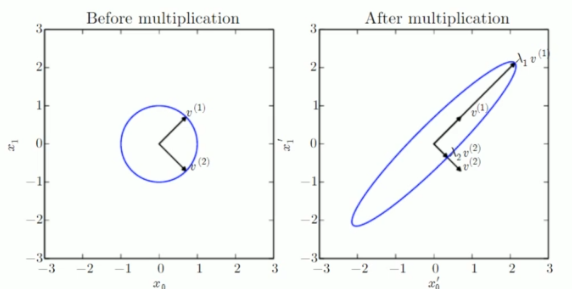
\includegraphics[width=0.8\textwidth]{gambar/gmb2.png}
    \caption{Perkalian antar dua buah vektor ortonormal eigen: $\mathbf{v^1}$ dan $\mathbf{v^2}$ dengan matriks $\mathbf{A}$ mengubah lingkaran satuan (\textit{unit circle}).}
    \label{fig:fig2}
\end{figure}

Dekomposisi eigen dimungkinkan jika matriks $\mathbf{A}$ mempunyai $n$ vektor - vektor eigen yang bersifat independen secara linier, sehingga kita dapat membentuk sebuah matriks $\mathbf{V}$ yang dengan sebuah vektor eigen per kolomnya dan sebuah vektor $\lambda$ yang memuat seluruh nilai - nilai eigen. Formulasi umum dari dekomposisi eigen untuk matriks $\mathbf{A}$ ditunjukkan pada persamaan \ref{eqn:eqn17} sebagai berikut:
\begin{equation}\label{eqn:eqn17}
    \mathbf{A} = \mathbf{V}\text{diag}(\lambda)\mathbf{V}^-1
\end{equation}

\subsection{Invers matriks}
Invers suatu matriks ($\mathbf{A}^{-1}$) digambarkan pada persamaan \ref{eqn:eqn18} berikut ini:

\begin{equation}\label{eqn:eqn18}
    \mathbf{A}.\mathbf{A}^{-1} = \mathbf{A}^{-1}.\mathbf{A} = \mathbf{I} 
\end{equation}
dimana $\mathbf{I}$ merupakan matriks identitas. Secara umum invers matriks ekuivalen dengan hubungan timbal-balik di dalam operasi perkalian di bilangan bulat.

\subsection{Sifat - sifat dekomposisi eigen}
Berikut adalah sifat - sifat dekomposisi eigen yang wajib kita pahami:


\begin{itemize}
    \item Dekomposisi eigen tidak dapat diterapkan pada seluruh matriks.
    \item Suatu matriks dikatakan matriks singular (tidak mempunyai invers) jika terdapat salah satu nilai eigen-nya yang bernilai nol.
    \item Suatu matriks yang mempunyai seluruh nilai eigen positif disebut sebagai definit positif.
    \item Suatu matriks yang mempunyai seluruh nilai eigen negatif disebut sebagai definit negatif.
\end{itemize}

\subsection{Motivasi penerapan dekomposisi eigen}
Dekomposisi eigen digunakan di dalam algoritma analisis komponen utama (\textit{Principle Component Analysis}: PCA). PCA merupakan prosedur statistik yang digunakan untuk mengubah suatu himpunan observasi dari variabel - variabel yang saling terkait menjadi suatu himpunan variabel yang secara linear tidak terkorelasi yang dinamakan komponen - komponen utama (\textit{principle components}). Secara umum dapat dikatakan bahwa PCA merupakan suatu metode yang digunakan untuk merangkum dan mengompresi data.

\section{Laboratorium 2: Norma dan dekomposisi eigen}
Pada catatan sebelumnya, kita telah membahas tentang konsep norma pada vektor dan matriks, normalisasi vektor, dan dekomposisi eigen. Pada bagian ini , kita akan menggunakan NumPy untuk mempermudah proses komputasinya dan memperkuat pemahaman kita akan konsep - konsep tersebut.

Seperti biasa, sebelum memulai kita harus memastikan bahwa kita menggunakan lingkungan komputasi yang sama:

\begin{pyin}
import sys
import numpy as np
from numpy import linalg

print('Python: {}'.format(sys.version))
print('NumPy: {}'.format(np.__version__))
\end{pyin}

\begin{pyout}
Python: 3.8.3 (default, May 19 2020, 18:47:26) 
[GCC 7.3.0]
NumPy: 1.18.1
\end{pyout}

\subsection{Norma vektor dan matriks}
Untuk menghitung norma vektor atau matriks, kita hanya cukup menggunakan satu baris perintah dengan fungsi \verb|linalg.norm()|:

\begin{pyin}
# mendefinisikan array
A = np.arange(9) - 3
A
\end{pyin}

\begin{pyout}
array([-3, -2, -1,  0,  1,  2,  3,  4,  5])
\end{pyout}

\begin{pyin}
# melakukan reshape membentuk matriks berukuran 3 x 3
B = A.reshape((3,3))
B
\end{pyin}

\begin{pyout}
array([[-3, -2, -1],
       [ 0,  1,  2],
       [ 3,  4,  5]])
\end{pyout}

\begin{pyin}
# Perhitungan Norma Euklidesan (L2)
print(np.linalg.norm(A))
print(np.linalg.norm(B))
\end{pyin}

\begin{pyout}
8.306623862918075
8.306623862918075
\end{pyout}

\begin{pyin}
# Perhitungan Norma Frobenius (L2 Norm untuk matriks)
print(np.linalg.norm(B, 'fro'))
\end{pyin}

\begin{pyout}
8.306623862918075
\end{pyout}

\begin{pyin}
# Perhitungan Norma L1
print(np.linalg.norm(A, 1))
print(np.linalg.norm(B, 1))
\end{pyin}

\begin{pyout}
21.0
8.0
\end{pyout}

\begin{pyin}
# Perhitungan norma maks (P = tak hingga)
print(np.linalg.norm(A, np.inf))
print(np.linalg.norm(B, np.inf))
\end{pyin}

\begin{pyout}
5.0
12.0
\end{pyout}

\subsection{Normalisasi vektor}
\begin{pyin}
# normalisasi untuk mendapatkan vektor satuan
norm = np.linalg.norm(A, 2)
sat_A = A / norm

print(sat_A)
\end{pyin}

\begin{pyout}
\%[-0.36115756 -0.24077171 -0.12038585  0.          0.12038585  0.24077171
  0.36115756  0.48154341  0.60192927]
\end{pyout}

\begin{pyin}
# norma dari vektor satuan adalah 1
np.linalg.norm(sat_A)
\end{pyin}

\begin{pyout}
1.0
\end{pyout}

\subsection{Dekomposisi eigen}
Kita dapat menghitung nilai dan vektor eigen dengan sangat mudah dengan menggunakan NumPy. Ingat bahwa vektor eigen dari matriks persegi $\mathbf{A}$ merupakan vektor bukan-nol $\mathbf{v}$, di mana perkalian dengan $\mathbf{A}$ hanya akan mengubah skalanya saja:

$$\mathbf{Av} = \lambda \mathbf{v}$$

Nilai skalar $\lambda$ dikenal sebagai nilai eigen.

\begin{pyin}
# mencari nilai dan vektor eigen untuk matriks persegi sederhana
A = np.diag(np.arange(1,4))
A
\end{pyin}

\begin{pyout}
array([[1, 0, 0],
       [0, 2, 0],
       [0, 0, 3]])
\end{pyout}

\begin{pyin}
nilai_eigen, vektor_eigen = np.linalg.eig(A)
print("Nilai - nilai eigen: {}".format(nilai_eigen))
print("Vektor - vektor eigen: {}".format(vektor_eigen))
\end{pyin}

\begin{pyout}
Nilai - nilai eigen: [1. 2. 3.]
Vektor - vektor eigen: [[1. 0. 0.]
 [0. 1. 0.]
 [0. 0. 1.]]
\end{pyout}

\begin{pyin}
# nilai eigen w[i] berkorespondensi pada vektor eigen v[:, i]
print('Nilai eigen: {}'.format(nilai_eigen[1]))
print('Vektor eigen: {}'.format(vektor_eigen[:,1]))
\end{pyin}

\begin{pyout}
Nilai eigen: 2.0
Vektor eigen: [0. 1. 0.]
\end{pyout}

Kita dapat dengan mudah melakukan pengecekan kembali pada nilai dan vektor eigen ini dengan melakukan perhitungan sebagai berikut:
 $$\textbf{A} = \textbf{V}diag(\lambda)\textbf{V}^{-1}$$
\begin{pyin}
# verifikasi - dekomposisi eigen untuk menghasilkan nilai A

matriks = np.matmul(np.diag(nilai_eigen), np.linalg.inv(vektor_eigen))
A = np.matmul(vektor_eigen, matriks).astype(np.int)
print(A)
\end{pyin}

\begin{pyout}
\%[[1 0 0]
 [0 2 0]
 [0 0 3]]
\end{pyout}

Nilai dan vektor eigen umumnya sulit untuk dipahami secara konseptual, untuk itu pada contoh berikut ini, kita mencoba memvisualisasikan perkalian antara vektor - vektor eigen dengan matriks $A$ dengan menggunakan pustaka matplotlib.

\begin{pyin}
# mengimpor pustaka - pustaka yang diperlukan untuk visualisasi data
import matplotlib.pyplot as plt
from mpl_toolkits.mplot3d import Axes3D
import matplotlib.cm as cm
\%matplotlib inline
\end{pyin}

\begin{pyin}
# plot vektor - vektor eigen
titik_awal = [0,0,0]

fig = plt.figure(figsize=(18,10))
ax1 = fig.add_subplot(121, projection='3d')

ax1.quiver(titik_awal, titik_awal, titik_awal, vektor_eigen[0, :], vektor_eigen[1, :], vektor_eigen[2, :], color = 'k')
ax1.set_xlim([-3, 3])
ax1.set_ylim([-3, 3])
ax1.set_zlim([-3, 3])
ax1.set_xlabel('sumbu-$x$')
ax1.set_ylabel('sumbu-$y$')
ax1.set_zlabel('sumbu-$z$')
ax1.view_init(15, 30)
ax1.set_title("Sebelum Perkalian")

# perkalian matriks awal dengan vektor - vektor eigen
eig_baru = np.matmul(A, vektor_eigen)
ax2 = plt.subplot(122, projection='3d')

# plot vektor - vektor baru
ax2.quiver(titik_awal, titik_awal, titik_awal, eig_baru[0, :], eig_baru[1, :], eig_baru[2, :], color = 'k')

# plot nilai - nilai eigen untuk setiap vektor 
ax2.plot((nilai_eigen[0]*vektor_eigen[0]), (nilai_eigen[1]*vektor_eigen[1]), (nilai_eigen[2]*vektor_eigen[2]), 'rX')
ax2.set_title("Sesudah Perkalian")
ax2.set_xlim([-3, 3])
ax2.set_ylim([-3, 3])
ax2.set_zlim([-3, 3])
ax2.set_xlabel('sumbu-$x$')
ax2.set_ylabel('sumbu-$y$')
ax2.set_zlabel('sumbu-$z$')
ax2.view_init(15, 30)

# tampilkan plot!
plt.show()
\end{pyin}

\begin{figure}[H]
    \centering
    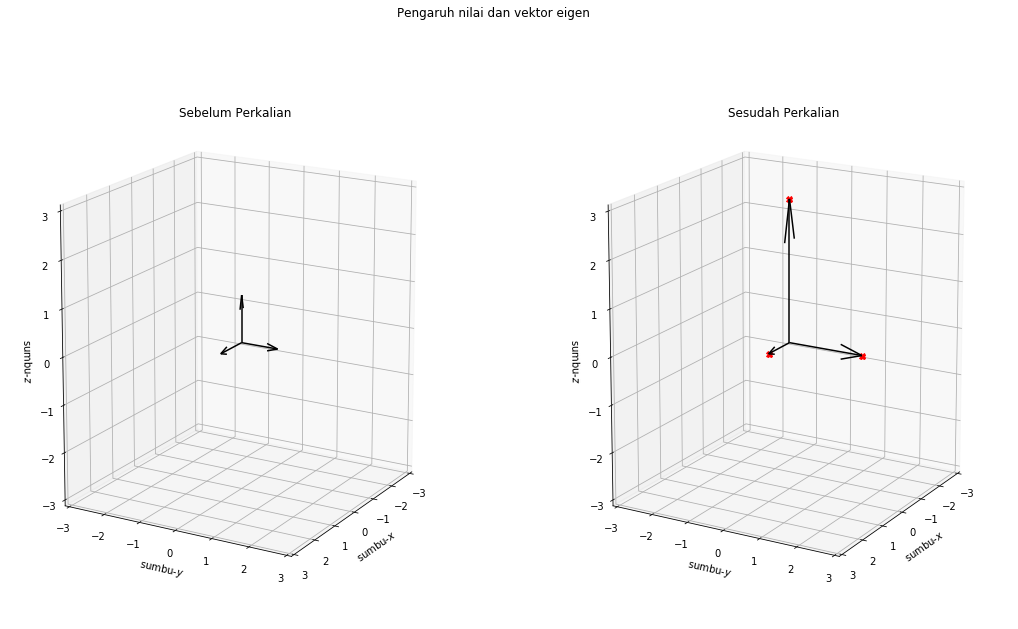
\includegraphics[width=1\textwidth]{gambar/gmb3.png}
    \caption{Pengaruh nilai dan vektor eigen.}
    \label{fig:fig3}
\end{figure}
\blankpage
\chapter{Kalkulus Peubah Banyak}
Turunan peubah banyak lazim digunakan untuk mengoptimisasi jaringan saraf tiruan dengan menggunakan berbagai algoritma yang masuk dalam kategori penurunan gradien (\textit{gradient descent}), utamanya dengan menggunakan algoritma penurunan gradien stokastik (\textit{stochastic gradient descent}) (Gambar \ref{fig:fig4}). Sementara integral digunakan untuk memahami distribusi probabilitas kontinyu dalam teori probabilitas. Bagian ini hanya akan membahas kulit luar konsep - konsep di dalam kalkulus karena sifatnya sebagai pengantar semata.

\begin{figure}[H]
    \centering
    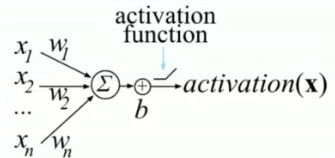
\includegraphics[width=0.5\textwidth]{gambar/gmb4.png}
    \caption{Optimasi algoritma jaringan saraf tiruan.}
    \label{fig:fig4}
\end{figure}

\section{Turunan}
Secara geometris turunan merupakan ukuran kemiringan dari suatu kurva atau yang sering disebut sebagai garis tangen. Kemiringan ini menyatakan ukuran perubahan kurva pada suatu titik tertentu. Sedangkan secara fisis, turunan merupakan laju perubahan suatu fungsi. Turunan satu dimensi dari fungsi $y=f(x)$ dinyatakan melalui notasi sebagai berikut(persamaan \ref{eqn:eqn19}):

\begin{dmath}\label{eqn:eqn19}
f'(x) = \frac{dy}{dx} = \frac{df(x)}{dx} = \frac{d}{dx}f(x)
\end{dmath}

Terdapat beberapa aturan di dalam penggunaan turunan di antaranya adalah sebagai berikut:
\subsection{Aturan turunan skalar}

\subsubsection{Konstanta}
Suatu konstanta karena sifatnya yang tetap, tidak akan pernah mengalami perubahan, maka berlaku:
\begin{equation}\label{eqn:eqn20}
    \frac{d}{dx} C = 0
\end{equation}
Contoh:
\begin{equation*}
    \frac{d}{dx}(128) = 0
\end{equation*}
\subsubsection{Aturan pangkat}
\begin{equation}\label{eqn:eqn21}
    \frac{d}{dx}x^{n} = nx^{n-1}
\end{equation}
Contoh:
\begin{equation*}
    \frac{d}{dx}x^{3} = 3x^{2}
\end{equation*}

\subsubsection{Perkalian}
\begin{equation}\label{eqn:eqn22}
    \frac{d}{dx}Cx^{n} = C\frac{d}{dx}x^{n} = Cx^{n-1}
\end{equation}
Contoh:
\begin{equation*}
    \frac{d}{dx}(4x^{3}) = 4\frac{d}{dx}x^{3} = 4(3)x^{2} = 12x^{2} 
\end{equation*}
\subsection{Aturan utama turunan}

\subsubsection{Aturan penjumlahan}
\begin{equation}\label{eqn:eqn23}
\frac{d}{dx}(f(x) + g(x)) = \frac{d}{dx} f(x) + \frac{d}{dx} g(x)    
\end{equation}
Contoh:
\begin{dmath*}
    \frac{d}{dx}(4x + 2x^{2}) = 4\frac{d}{dx}x^{2} + 2\frac{d}{dx}x^{2} = 4 + 4x
\end{dmath*}
\subsubsection{Aturan perkalian}
\begin{equation}\label{eqn:eqn24}
    \frac{d}{dx}(f(x).g(x)) = g(x)\frac{d}{dx}f(x) + f(x)\frac{d}{dx}g(x)
\end{equation}
Contoh:
\begin{dmath*}
    \frac{d}{dx}(x^{2}x) = x\frac{d}{dx}x^{2} + x^{2} \frac{d}{dx}x = x(2x) + x^{2} = 3x^{2}
\end{dmath*}

\sububsection{Aturan rantai}
Aturan ini penting untuk dipahami karena banyak digunakan di dalam analisis jaringan saraf tiruan.
\begin{equation}\label{eqn:eqn25}
    \frac{d}{{dx}}\left[ {f\left( u \right)} \right] = \frac{d}{{du}}\left[ {f\left( u \right)} \right]\frac{{du}}{{dx}}
\end{equation}
Contoh:
\begin{dmath*}
\frac{d}{dx}\sin{(x^{2})} = \cos{(x^2)}.2x = 2x\cos{(x^2)}
\end{dmath*}
\sububsection{Mengenal turunan parsial}
Turunan parsial digunakan untuk menyelesaikan permasalahan turunan yang melibatkan lebih dari satu peubah. Turunan parsial dua dimensi dinyatakan sebagai berikut(persamaan \ref{eqn:eqn26}):
\begin{equation}\label{eqn:eqn26}
    f'(x,y) = \nabla f(x,y) = \left[\frac{\partial f(x,y)}{\partial x}, \frac{\partial f(x,y)}{\partial y}\right]  
\end{equation}
Contoh:
\begin{eqnarray*}
f(x,y) = 3x^{2}y\\
\nabla f(x,y) = \left[\frac{\partial(3x^{2}y)}{\partial x}, \frac{\partial (3x^{2}y)}{\partial y} \right] = \left[3y(2x), 3x^{2}(1)\right] = \left[6xy, 3x^{2}\right]
\end{eqnarray*}

\section{Integral}
Konsep integral banyak digunakan untuk pemodelan distribusi probabilitas kontinyu yang digunakan dalam berbagai algoritma pemelajaran mesin. Metode integrasi umumnya digunakan untuk mencari luasan wilayah di bawah kurva (Gambar \ref{fig:fig5}). Proses integrasi merupakan kebalikan dari diferensiasi (turunan), maka integral sering dikenal sebagai anti-turunan. Formulasi umum integral ditunjukkan pada persamaan \ref{eqn:eqn27} berikut ini:
\begin{equation}\label{eqn:eqn27}
\int f'(x) dx = f(x) + C
\end{equation}
, dimana $C$ merupakan konstanta integrasi.

\begin{figure}[H]
    \centering
    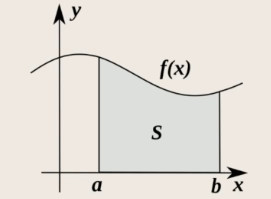
\includegraphics[width=0.5\textwidth]{gambar/gmb5.png}
    \caption{Ilustrasi integral untuk mencari luasan di bawah kurva.}
    \label{fig:fig5}
\end{figure}

\subsection{Jenis - jenis integral}
Terdapat dua jenis integral, yakni:
\subsubsection{Integral tak-tentu}
Integral tanpa batas yang diformulasikan sebagai berikut:
\begin{equation}\label{eqn:eqn28}
    \int f(x) dx
\end{equation}
\sububsection{Integral tentu}
Integral yang mempunyai batasan tertentu yang diformulasikan sebagai berikut:
\begin{equation}\label{eqn:eqn28}
    \int_{a}^{b} f(x) dx
\end{equation} 

\subsection{Aturan integral}
\subsubsection{Aturan pangkat}
\begin{equation}\label{eqn:eqn29}
    \int x^{n} dx = \frac{x^{n + 1}}{n + 1} + C
\end{equation}
Contoh:
\begin{equation*}
    \int x^{2} = \frac{x^3}{3} + C
\end{equation*}
\subsubsection{Aturan konstanta}
\begin{equation}\label{eqn:eqn30}
    \int k dx = kx + C
\end{equation}
Contoh:
\begin{equation*}
    \int 4 dx = 4x + C
\end{equation*}
\subsection{Penyelesaian integral tentu}
Berikut ini merupakan algoritma yang umum digunakan untuk menyelesaikan integral tentu:
\begin{dmath}\label{eqn:eqn31}
\int_{a}^{b} f'(x) dx = f(x)\big|_{a}^{b} = f(b) - f(a)
\end{dmath}
Contoh:
\begin{equation*}
\int_{0}^{2} 3x^{2} dx = 3 \int_{0}^{2} x^{2} dx = 3\left(\frac{x^3}{3}\right) \Big|_0^{2} = x^{3} \Big|_{0}^{2} = (2)^{3} - (0)^{3} = 8    
\end{equation*}
\section{Gradien}
Gradien umum digunakan untuk mengoptimasi algoritma jaringan saraf tiruan. Konsep gradien pada dasarnya berangkat dari turunan parsial yang seperti telah bersama kita ketahui dapat diorganisasikan ke dalam bentuk vektor(persamaan \ref{eqn:eqn32} merupakan contoh implementasi gradien pada dimensi tiga).

\begin{equation}\label{eqn:eqn32}
\nabla f(x,y) = \left[\frac{\partial f(x,y,z)}{\partial x}, \frac{\partial f(x,y,z)}{\partial y}, \frac{\partial f(x,y,z)}{\partial z}\right]
\end{equation} 

Seperti juga turunan, gradien merepresentasikan derajat kemiringan dari suatu fungsi. Gradien mengarah pada arah laju perubahan terbesar pada fungsi, dan besarannya menyatakan kemiringan pada arah tersebut. Dengan demikian gradien sangatlah cocok untuk digunakan untuk meminimalkan fungsi kerugian pada banyak algoritma pemelajaran mesin. Gradien tidak hanya terbatas pada dimensi tiga, kita dapat melakukan ekspansi pada dimensi - dimensi yang lebih besar seperti yang umum dilakukan ketika menerapkan algoritma pemelajaran mesin pada data raksasa.

Vektor gradien digunakan untuk menyusun turunan - turunan parsial dari suatu fungsi skalar. Ketika gradien diterapkan pada banyak fungsi, maka didefinisikan ke dalam bentuk matriks Jacobian. Formulasi matriks Jacobian untuk dua fungsi dengan dua buah peubah ditampilkan pada persamaan \ref{eqn:eqn33} sebagai berikut:

\begin{equation}\label{eqn:eqn33}
J = \begin{bmatrix}\nabla f(x,y) \\ \nabla g(x,y)\end{bmatrix} = \begin{bmatrix}\frac{\partial f(x,y)}{\partial x} & \frac{\partial f(x,y)}{\partial y} \\ \frac{\partial g(x,y)}{\partial x} & \frac{\partial g(x,y)}{\partial y} \end{bmatrix}
\end{equation} 

Formulasi umum untuk kasus dengan:
\begin{dmath*}
f(\mathbf{x}) = f(x_{1}, x_{2}, \cdots , x_{n}) 
\end{dmath*}
, adalah sebagai berikut (persamaan \ref{eqn:eqn34})

\begin{equation}\label{eqn:eqn34}
J = \begin{bmatrix} \nabla f_{1}(\mathbf{x})\\\nabla f_{2}(\mathbf{x})\\ \vdots \\ \nabla f_{m}(\mathbf{x})\end{bmatrix} = \begin{bmatrix} \frac{\partial f_{1}(\mathbf{x})}{\partial x_{1}} & \frac{\partial f_{1}(\mathbf{x})}{\partial x_{2}} & \cdots & \frac{\partial f_{1}(\mathbf{x})}{\partial x_{n}}\\ \frac{\partial f_{2}(\mathbf{x})}{\partial x_{1}} & \frac{\partial f_{2}(\mathbf{x})}{\partial x_{2}} & \cdots & \frac{\partial f_{2}(\mathbf{x})}{\partial x_{n}}\\ \cdots & \cdots & \cdots & \cdots\\\frac{\partial f_{m}(\mathbf{x})}{\partial x_{1}} & \frac{\partial f_{m}(\mathbf{x})}{\partial x_{2}} & \cdots & \frac{\partial f_{m}(\mathbf{x})}{\partial x_{n}}\end{bmatrix}
\end{equation}

\section{Laboratorium 3: Visualisasi gradien menggunakan matplotlib}
Pada bagian ini kita hendak melakukan visualisasi gradien untuk persamaan 2D.

Disini kita hendak berfokus pada pemahaman algoritma gradien, namun kita juga akan mempelajari beberapa konsep \textit{scripting} dengan menggunakan Python. Konsep - konsep tersebut antara lain adalah penggunaan \textit{meshgrid} yang sangat berguna untuk menampilkan informasi yang berhubungan dengan titik - titik berbeda di dalam suatu \textit{array}. Selain itu, kita juga akan mempelajari tentang pustaka matplotlib dengan menggunakan plot \textit{quiver} dan \textit{pcolor}.

\begin{pyin}
import sys
import numpy as np
import matplotlib
import matplotlib.pyplot as plt

print('Python: {}'.format(sys.version))
print('NumPy: {}'.format(np.__version__))
print('Matplotlib: {}'.format(matplotlib.__version__))
\end{pyin}

\begin{pyout}
Python: 3.8.3 (default, May 19 2020, 18:47:26) 
[GCC 7.3.0]
NumPy: 1.18.1
Matplotlib: 3.2.1
\end{pyout}

Sel di atas digunakan untuk mengimpor beberapa pustaka yang kita gunakan dalam sesi komputasi ini. 

Dengan menggunakan NumPy, kita membuat sebuah meshgrid untuk setiap titik $x$ dan $y$. \textit{Meshgrid} ini merupakan \textit{array} dua dimensi yang akan kita gunakan untuk visualisasi. Nilai $z$ pada setiap titik $x$ dan $y$ dihitung dengan menggunakan fungsi sebagai berikut:

\begin{pyin}
# menghasilkan meshgrid 2D
nx, ny = (100, 100)

x = np.linspace(0, 10, nx)
y = np.linspace(0, 10, ny)

xv, yv = np.meshgrid(x,y)

# mendefinisikan fungsi untuk plotting
def f(x,y):
    return x * (y**2)

# menghitung nilai z untuk setiap titik x,y
z = f(xv, yv)
\end{pyin}

Sekarang kita telah mempunyai \textit{meshgrid} dan telah menghitung $f(x,y)$ untuk seluruh titik di \textit{meshgrid}. Saatnya untuk memvisualisasikan hasilnya melalui \textit{colormap}.

\begin{pyin}
# Membuat colorplot untuk menampilkan data 
plt.figure(figsize=(14,12))
plt.pcolor(xv, yv, z)
plt.colorbar()
plt.show()
\end{pyin}

\begin{figure}[H]
    \centering
    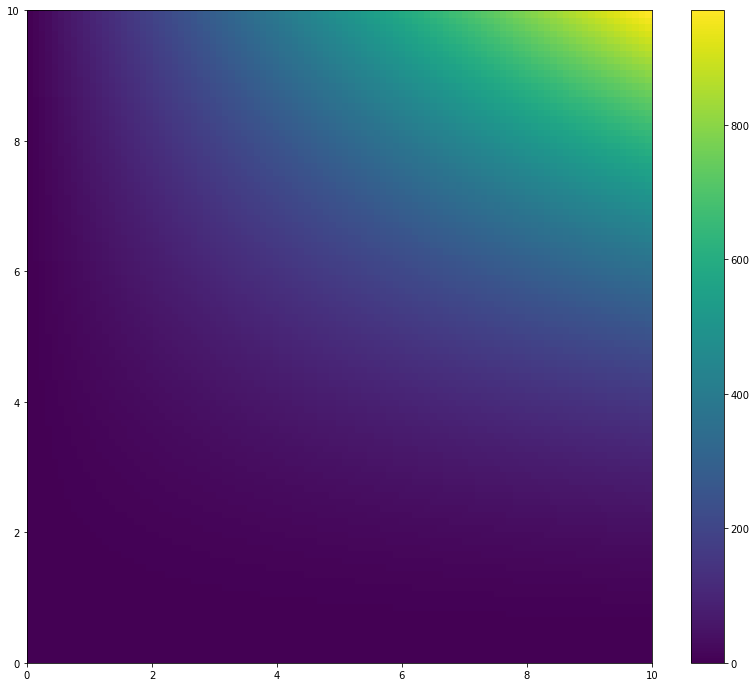
\includegraphics[width=0.5\textwidth]{gambar/gmb6.png}
    \caption{\textit{Colorplot} 2D dari fungsi $f(x,y)=xy^2$.}
    \label{fig:fig6}
\end{figure}

Sekarang saatnya kita menambahkan gradien ke dalam plot tersebut. Kita tidak akan menghitung gradien untuk setiap titik di dalam grafik ini, kita akan mendefinisikan \textit{meshgrid} baru dengan titik - titik yang lebih sedikit. Kita dapat memanfaatkan fungsi \verb|gradient()| di dalam pustaka NumPy untuk menghitung gradien pada setiap titik. Di sini kita harus berhati - hati karena prinsip kerja NumPy berbasis \textit{array}, maka luaran dari fungsi ini berupa baris, kolom bukan dalam format $x,y$.

\begin{pyin}
# membuat meshgrid 2D untuk gradien
nx, ny = (10, 10)
x = np.linspace(0, 10, nx)
y = np.linspace(0, 10, ny)
xg, yg = np.meshgrid(x,y)

# menghitung gradien untuk fungsi f(x,y)
# Catatan: NumPy menghasilkan luaran dalam format baris (y), kolom(x)
Gy, Gx = np.gradient(f(xg, yg))
\end{pyin}

Kemudian kita memvisualisasikan gradien menggunakan \textit{quiverplot} (Gambar \ref{fig:fig7}). Arah gradien direpresentasikan melalui anak panah, sedangkan besarannya direpresentasikan oleh panjang panah.

\begin{pyin}
# Memvisualisasikan gradien dengan colorplot
plt.figure(figsize=(14,12))
plt.pcolor(xv, yv, z)
plt.colorbar()
plt.quiver(xg, yg, Gx, Gy, scale = 1000, color = 'w')
plt.show()
\end{pyin}

\begin{figure}[H]
    \centering
    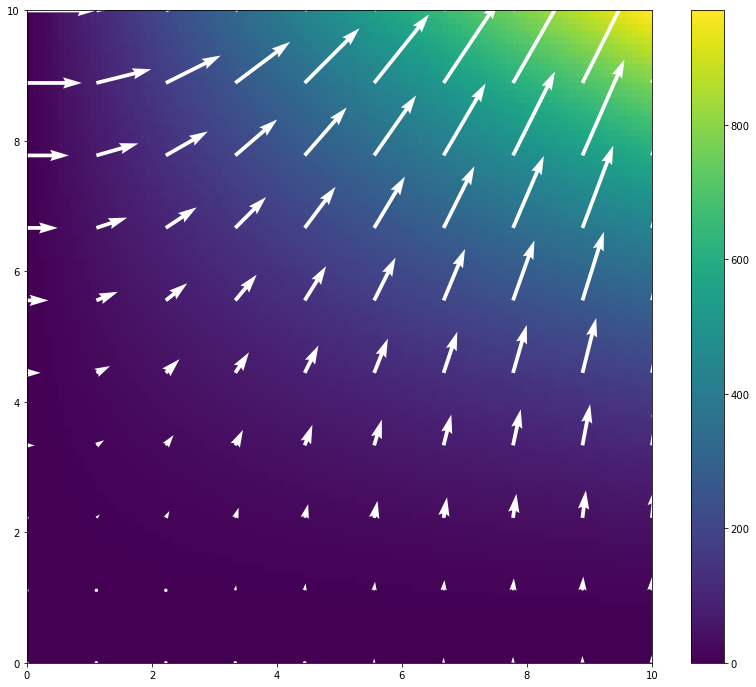
\includegraphics[width=0.5\textwidth]{gambar/gmb7.png}
    \caption{Gradien dari fungsi $f(x,y)=xy^2$.}
    \label{fig:fig7}
\end{figure}

\begin{pyin}
# Memvisualisasikan gradien dengan colorplot
plt.figure(figsize=(14,12))
plt.pcolor(xv, yv, z)
plt.colorbar()
plt.quiver(xg, yg, Gx, Gy, scale = 1000, color = 'w')
#plt.title('Gradient of f(x,y) = xy^2')
plt.show()
\end{pyin}

Plot di atas nampak sempurna. Anak - anak panah-nya nampak mengarah ke titik maksimum dan besarannya sesuai dengan kemiringan di setiap lokasi. Namun bagaimana kita bisa tahu kalau NumPy telah melakukan kalkulasi dengan benar? Untuk itu kita harus mencari turunan parsial melalui persamaan:

$$\nabla f(x,y) = \begin{bmatrix} \frac{d}{dx}f(x,y) && \frac{d}{dy}f(x,y) \end{bmatrix}$$

$$\nabla f(x,y) = \begin{bmatrix}y^2&&2xy\end{bmatrix}$$

Dengan mendefinisikan fungsi sebagai berikut:

\begin{pyin}
# menghitung gradien fungsi: f(x,y) = xy^2
def ddx(x,y):
    return y ** 2

def ddy(x,y):
    return (2 * y * x)

Gx = ddx(xg,yg)
Gy = ddy(xg,yg)
\end{pyin}

Kemudian kita memvisualisasikannya (Gambar \ref{fig:fig8}):

\begin{pyin}
# Plot
plt.figure(figsize=(14,12))
plt.pcolor(xv, yv, z)
plt.colorbar()
plt.quiver(xg, yg, Gx, Gy, scale = 1000, color = 'w')
plt.show()
\end{pyin}

\begin{figure}[H]
    \centering
    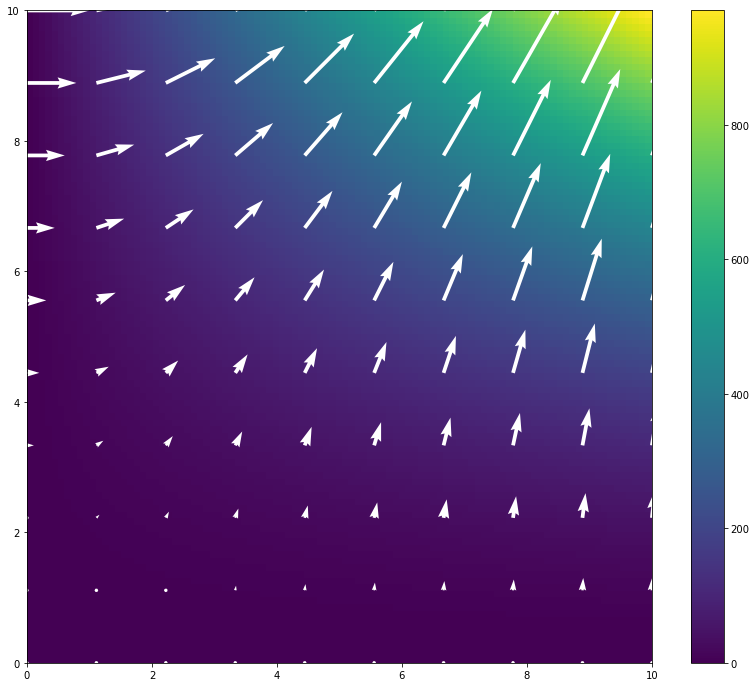
\includegraphics[width=0.5\textwidth]{gambar/gmb8.png}
    \caption{Visualisasi [$y^2$, $2xy$].}
    \label{fig:fig8}
\end{figure}

\section{Optimasi}
Pada bagian ini kita akan menggabungkan beberapa konsep yang telah kita pelajari pada bagian - bagian sebelumnya untuk memahami permasalahan optimasi pada fungsi konveks satu dimensi. Di dunia nyata tentunya kita akan disuguhkan oleh perkara optimasi yang melibatkan banyak dimensi, hanya karena buku ini hanya berupa pengantar matematis singkat, maka yang dibahas hanya pada perkara optimasi fungsi konveks berdimensi tunggal.  

Persamaan \ref{eqn:eqn35} menunjukkan formulasi umum dari optimasi fungsi konveks:

\begin{mini}|s|
{x}{f_{0}(x)}
{}{}
\addConstraint{f_{i}(x) \leq 0, i =\{i, \cdots, k\}}
\addConstraint{h_{j}(x) = 0, j = \{1,\cdots, k\}}
\label{eqn:eqn35}
\end{mini}
Berikut adalah beberapa terminologi yang wajib kita pahami:
\begin{itemize}
    \item $f_{0}(x)$: merupakan fungsi objektif yang hendak kita minimalkan (dalam kasus pemelajaran mesin merupakan fungsi kerugian).
    \item $x$: merupakan peubah objektif, umumnya di dalam algoritma jaringan saraf tiruan merupakan vektor masukan yang hendak kita \textit{update}.
    \item $f_{i}(x)$ dan $h_{j}(x)$ merupakan fungsi - fungsi kendala (\textit{constraint functions}) yang bentuknya dapat beragam.
\end{itemize}

Optimasi digunakan untuk mencari titik minimum global (Gambar \ref{fig:fig9}) dari suatu fungsi objektif yang mana harus memenuhi beberapa fungsi kendala.

\begin{figure}[H]
    \centering
    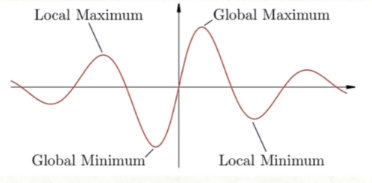
\includegraphics[width=0.7\textwidth]{gambar/gmb9.png}
    \caption{Visualisasi titik - titik kritis dari suatu fungsi objektif.}
    \label{fig:fig9}
\end{figure}

Jika fungsi objektif berupa fungsi konveks (cembung atau cekung), maka permasalahan optimasinya juga dikenal sebagai optimasi konveks. Pada fungsi konveks titik minimum yang hendak kita optimasi sudah pasti berupa titik minimum global.

Optimasi merupakan topik yang sangat penting di dalam analisis data karena hampir digunakan pada seluruh algoritma pemelajaran mesin, beberapa di antaranya adalah:
\begin{itemize}
    \item \textbf{Klasifikasi}:
    \begin{equation}
        \displaystyle{\minimize_{w} \sum_{i=1} \log(1 + \exp(-y_{i}x_{i}^{T}w)}
        \label{eqn:eqn36}
    \end{equation}
    \item \textbf{K-means}:
    \begin{equation}
        \displaystyle{\minimize_{\mu_{1}, \cdots, \mu_{k}}J(\mu) = \sum_{j=1}^{k}\sum_{i\in C_{j}}\lVert x_{i} - \mu_{j}\rVert^{2}}
        \label{eqn:eqn37}
    \end{equation}
    \item \textbf{Regresi logistik}:
    \begin{equation}
        \displaystyle{\minimize_{w} \lVert X_{w} - y \rVert^{2}}
        \label{eqn:eqn38}
    \end{equation}
\end{itemize}

Untuk lebih memahami persoalan optimasi ini kita akan mencoba menggunakan konsep turunan untuk mencari titik - titik kritis dari fungsi objektif $y = x^{2} + 3$ (Gambar \ref{fig:fig10}) dengan menggunakan turunan pertama dan kedua.
\begin{figure}[H]
    \centering
    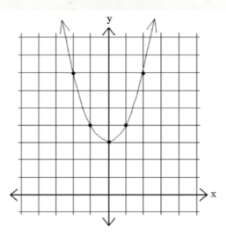
\includegraphics[width=0.5\textwidth]{gambar/gmb10.png}
    \caption{Fungsi  $y = x^{2} + 3$.}
    \label{fig:fig10}
\end{figure}

Yang pertama kali harus kita lakukan adalah mencari titik kritis dengan mengatur turunan pertama sama dengan nol:
\begin{equation*}
    y = x^{2} + 3
\end{equation*}
\begin{equation*}
    y' = 2x
\end{equation*}
\begin{equation*}
    0 = 2x
\end{equation*}
\begin{equation*}
    x = 0
\end{equation*}
Maka kita telah mengetahui titik kritis globalnya (karena fungsi ini merupakan fungsi konveks, maka seluruh titik kritisnya berlaku global). Untuk menguji apakah titik ini titik maksimum atau minimum, kita perlu melakukan penurunan kedua, yakni:
\begin{equation*}
    y'' = 2
\end{equation*}
Jika penurunan kedua bersifat positif, maka titik tersebut merupakan titik minimum, sedangkan jika bersifat negatif maka titik tersebut merupakan titik maksimum. Dalam kasus ini, maka titik minimum global dari fungsi $y = x^{3} + 3$ adalah $x = 0$.

Pencarian titik minimum global secara matematis tersebut umumnya tidak berlaku dalam konteks pemelajaran mesin. Karena volume data yang berjumlah sangat besar, maka diperlukan proses iteratif dengan menggunakan gradien. Jika gradien bernilai positif, maka kita menggeser ke arah lain hingga mendapatkan gradien yang bernilai negatif, dan hal ini dilakukan secara berulang hingga menemukan titik minimum yang dicari. Berikut ini contoh kasus yang mungkin dilakukan oleh algoritma pemelajaran mesin untuk mencari titik minimum:

\begin{enumerate}
    \item Tebakan pertama: $x=3$ merupakan titik minimum.
    \item Evaluasi $f(x)$:
    \begin{equation*}
        y = (3)^{2} + 3 = 12
    \end{equation*}
    \item Evaluasi nilai dari turunan:
    \begin{equation*}
        y' = 2(3) = 6
    \end{equation*}
    Ternyata gradien bernilai positif, maka kita harus mengubah arah tebakan.
    \item Tebakan kedua: $x = -1$ merupakan nilai minimum.
    \item Evaluasi $f(x)$:
        \begin{equation*}
           y = (-1)^{2} + 3 = 4
        \end{equation*}
    \item Evaluasi nilai dari turunan:
    \begin{equation*}
        y' = 2(-1) = -2
    \end{equation*}
    Ternyata tebakannya \textit{overshot}, maka kita ubah lagi arah tebakan.
    \item Begitu seterusnya hingga kita menemukan nilai $x = 0$ sebagai titik minimum.
\end{enumerate}

Proses ini dinamakan sebagai optimasi gradien stokastik. Pada algoritma jaringan saraf tiruan, jarak yang digunakan untuk mengubah arah tebakan umumnya tidak sebesar contoh di atas (dari 3 ke -2), melainkan sangatlah kecil (dari 3 ke 2,99 misalnya). Oleh karena volume data yang umumnya sangat besar, proses iterasi ini dapat berlangsung hingga ribuan, bahkan jutaan kali. 

Di dalam dunia nyata tentu tidak seluruh fungsi objektif yang hendak kita optimasi merupakan fungsi konveks, sehingga kita harus memperhitungkan juga titik - titik kritis yang bersifat lokal.
\blankpage
\chapter{Teori Probabilitas}
\section{Pendahuluan}
Teori probabilitas digunakan untuk mengkuantifikasikan ketidakpastian. Teori probabilitas menyediakan aksioma - aksioma yang dapat digunakan untuk menurunkan pernyataaan - pernyataan matematis tentang ketidakpastian.

Di bidang analisis data sendiri, hukum - hukum probabilitas digunakan sebagai fondasi tentang bagaimana suatu sistem algoritma menimbang permasalahan dan memberikan keputusan untuk menyelesaikan permasalahan tersebut. Dapat dikatakan bahwa teori probabilitas merupakan batu penjuru dari kemampuan dari suatu sistem kecerdasan buatan untuk dapat berpikir dan menimbang permasalahan selayaknya manusia biasa yang kesehariannya tidak luput dari ketidakpastian.

Terdapat tiga macam sumber ketidakpastian ketika kita hendak menganalisis data, yakni:
\begin{itemize}
	\item Ketidakpastian stokastik yang bersifat inheren, yakni secara natural sistem yang hendak kita modelkan diatur oleh hukum - hukum alam yang bersifat tidak pasti. Contoh yang paling terkenal adalah pemodelan mekanika kuantum.
	\item Ketidaklengkapan hasil observasi. Dalam kasus ini kita tidak mempunyai seluruh data yang hendak dimodelkan. Jenis ketidakpastian inilah yang utamanya sering dijumpai ketika kita melakukan penganalisisan data. Misalnya, ketika kita hendak menerapkan algoritma pengenalan objek - objek lalulintas pada mobil swakemudi, tentu kita hanya melatih sistem tersebut dengan ratusan (atau bahkan ribuan) objek - objek fotografi rambu - rambu lalulintas, sedangkan pada kenyataannya mobil swakemudi ini harus berhadapan dengan seluruh rambu - rambu lalulintas di seluruh jalan raya di Indonesia.
	\item Ketidaklengkapan pemodelan. Seringkali karena keterbatasan sumberdaya komputasi kita hanya memodelkan beberapa fitur penting saja, sehingga beberapa fitur yang mendetail sengaja kita abaikan karena keterbatasan sumberdaya komputasi. Salah satu contohnya adalah pemodelan iklim global yang mungkin saja gagal menangkap fenomena regional seperti sistem monsun.
\end{itemize} 

Oleh karena tiga ketidakpastian tersebut, kita membutuhkan teori probabilitas untuk memodelkan data yang telah kita peroleh. 

Berdasarkan kesepakatan para ilmuwan, teori probabilitas terbagi ke dalam dua mazhab utama, yakni:
\begin{itemize}
	\item Probabilitas frekuensi, yang mana lebih menekankan pada frekuensi terjadinya suatu kejadian tertentu. Contohnya adalah seberapa sering kita memperoleh dadu dengan jumlah enam ketika dua kali melemparkan dadu.
	\item Probabilitas Bayesian, yang mana lebih menekankan pada derajat kepercayaan. Contohnya adalah ketika dokter menyatakan seorang pasien mempunyai 40\% peluang terjangkit COVID-19.
\end{itemize}
\section{Distribusi - distribusi probabilitas}
\subsection{Peubah acak}
Peubah acak (\textit{random variable}) merupakan suatu peubah yang dapat memperoleh nilai secara acak dari suatu himpunan nilai. Peubah acak $X$ dapat memperoleh nilai dari himpunan bilangan $\{x_{1}, x_{2}, x_{3}, \cdots, x_{n}\}$. Distribusi probabilitas sendiri bertugas untuk menentukan seberapa besar peluang suatu nilai di dalam himpunan bilangan yang dimaksud untuk terpilih sebagai peubah acak. Terdapat dua jenis peubah acak, yakni:
\begin{itemize}
\item \textbf{Diskrit}, yang mana mempunyai nilai - nilai tertentu (bersifat finit), dan
\item \textbf{Kontinyu}, yang mana himpunan kandidat peubah acak tersebut merupakan bilangan riil yang bersifat kontinyu.
\end{itemize} 

\subsection{Fungsi massa peluang} 
Distribusi probabilitas untuk peubah acak diskrit dikenal sebagai fungsi massa peluang (\textit{Probability Mass Function}: PMF). Terdapat tiga kriteria yang menyatakan bahwa suatu fungsi dapat dikategorikan sebagai PMF:
\begin{itemize}
\item Domain dari $P$ harus memenuhi setiap nilai dari $x$.
\item $0 \leq P(X) \leq 1$
\item $\Sigma P(X) = 1$, oleh karena itu distribusi probabilitas pada PMF selalu ternormalisasi.
\end{itemize}

Terdapat dua jenis PMF, yakni:
\begin{itemize}
	\item Distribusi probabilitas gabungan, yang mana merupakan PMF yang berlaku pada banyak peubah. $P(X=x, Y=y)$ berlaku untuk setiap $X=x$ dan $Y=y$ secara bersamaan.
	\item  Distribusi seragam, pada distribusi ini seluruh elemen di dalam himpunan peubah acak mempunyai peluang yang sama untuk terpilih. Berikut adalah formulasi umumnya (persamaan \ref{eqn:eqn39}):
	\begin{equation}\label{eqn:eqn39}
	P(X=x_{i}) = \frac{1}{k}
	\end{equation}
Untuk kasus PMF sendiri akan lebih mudah dihitung karena mempunyai nilai - nilai yang bersifat diskrit:

\begin{equation*}
\sum_{i}P(X=x_{i}) = \sum_{i}\frac{1}{k} = \frac{k}{k} = 1
\end{equation*}
\end{itemize}

\subsection{Fungsi kepadatan peluang}
Fungsi kepadatan peluang (\textit{Probability Density Function}: PDF) banyak dijumpai di dalam riset - riset tentang kecerdasan buatan. PDF berlaku pada peubah acak yang bersifat kontinyu.
Terdapat tiga kriteria yang menyatakan bahwa suatu fungsi dapat dikategorikan sebagai PMF:

\begin{itemize}
\item Domain dari $p$ harus memenuhi setiap nilai dari $x$.
\item $p(x) \geq 0$
\item $\int p(x) dx = 1$
\end{itemize}

\subsection{Probabilitas marjinal}
Merupakan distribusi probabilitas bagian dari seluruh peubah. Jenis probabilitas ini banyak dijumpai di dalam kegiatan analisis data karena umumnya kita tidak mempunyai seluruh peubah yang dibutuhkan untuk implementasi pemelajaran mesin. Berikut ini formulasi umum probabilitas marjinal:
\begin{itemize}
    \item Peubah acak diskrit:
    \begin{equation}
        P(X=x) = \sum_{y} P(X=x, Y=y)
        \label{eqn:eqn40}
    \end{equation}
    \item Peubah acak kontinyu:
    \begin{equation}
        p(x) = \int p(x,y) dy
        \label{eqn:eqn41}
    \end{equation}
\end{itemize}
\subsection{Probabilitas bersyarat}
Probabilitas bersyarat adalah probabilitas dari suatu kejadian yang bergantung pada kejadian lainnya. Formulasi umumnya dapat dilihat pada persamaan \ref{eqn:eqn42}:
\begin{equation}
    P(Y=y | X=x) = \frac{P(Y=y, X=x)}{P(X=x)}
    \label{eqn:eqn42}
\end{equation}

\section{Ekspektasi, varian, dan kovarian}
\subsection{Ekspektasi}
Ekspektasi dari suatu fungsi $f(x)$ dengan mempertimbangkan distribusi probabilitas $P(x)$ merupakan nilai rata - rata ketika kita melakukan eksperimen terhadap $x$ pada distribusi $P$. Berikut adalah formulasi umum ekspektasi pada:
\begin{itemize}
	\item Peubah acak diskrit: 
	\begin{equation}\label{eqn:eqn43}
		E_{x \sim\ p}\left[f(x)\right] = \sum_{x} P(x)f(x)
	\end{equation}
	\item Peubah acak kontinyu:
	\begin{equation}\label{eqn:eqn44}
		E_{x \sim\ p}\left[f(x)\right] = \int p(x) f(x) dx
	\end{equation}
\end{itemize}
\subsection{Varian dan standar deviasi}
Secara formal varian $(\sigma^2)$ berarti ekspektasi dari kuadrat deviasi peubah acak dari rata - ratanya. Secara informal varian dapat dikatakan sebagai ukuran seberapa jauh bilangan acak yang diambil dari distribusi probabilitas $P(x)$ menyebar dari nilai rata - ratanya. Berikut merupakan formulasi umum varian (persamaan \ref{eqn:eqn45}):
\begin{equation}
    \text{Var}(f(x)) = E\left[(f(x) - E[f(x)])^2\right]
    \label{eqn:eqn45}
\end{equation}
Sementara itu, standar deviasi $(\sigma)$ tidak lain merupakan akar kuadrat dari varian.
\subsection{Kovarian}
Kovarian merupakan ukuran keterkaitan linier antara dua peubah acak (persamaan \ref{eqn:eqn46}):
\begin{equation}
    \text{Cov}(f(x), g(y)) = E\left[f(x) -E[f(x)]\right](g(y) - E[g(y)])
    \label{eqn:eqn46}
\end{equation}
Kovarian digunakan untuk mengukur dependensi linier antar peubah.
\section{Matriks kovarian}
Matriks kovarian dari vektor acak $\mathbf{x}$ merupakan matriks $n \times n$, di mana berlaku:
\begin{equation}
    \text{Cov}(\mathbf{x})_{i,j} = \text{Cov}(x_{i}, x_{j})
    \label{eqn:eqn47}
\end{equation}
Elemen - elemen pada diagonal matriks kovarian merupakan varian:
\begin{equation}
    \text{Cov}(x_{i}, x_{i}) = \text{Var}(x_{i})
    \label{eqn:eqn48}
\end{equation}
Ketika berbicara mengenai varian di dalam ranah pemelajaran mesin, maka umumnya kita akan mengacu matriks kovarian.

\section{Laboratorium 4: Visualisasi distribusi probabilitas}
Pastikan kalian memulai laboratorium ini dengan memilih kernel R pada Jupyter Notebook kalian masing - masing.

Contoh yang akan kita gunakan di dalam kegiatan kali ini adalah tentang IQ siswa dengan rata - rata: 100 dan standar deviasi: 15. Yang menjadi pertanyaan adalah berapa persen siswa dengan IQ $> 115$?

Mendefinisikan parameter untuk distribusi normal:

\begin{verbatim}
rata2 <- 100
std <- 15
\end{verbatim}

Mendefinisikan batas atas dan batas bawah \textit{Region of Interest} (ROI):

\begin{verbatim}
bawah <- 115
atas <- Inf
\end{verbatim}

Membuat sikuen bilangan dan distribusi normal:

\begin{verbatim}
x <- seq(-4,4, length = 100) * std + rata2
prob <- dnorm(x, rata2, std)
\end{verbatim}

Memvisualisasikan distribusi probabilitas dan menambahkan label sumbu:

\begin{verbatim}
plot(x,prob,
     type="n", 
     xlab="Skor IQ",
     ylab="p(x)",
     main="Distribusi normal skor IQ", axes=FALSE)
lines(x,prob)
axis(1, at=seq(40, 160, 20), pos=0)
\end{verbatim}

Mendefinisikan poligon untuk ROI:

\begin{verbatim}
plot(x,prob, type="n", xlab="Skor IQ", 
     ylab="p(x)", 
     main="Distribusi normal skor IQ",
     axes=FALSE)
lines(x,prob)
axis(1, at=seq(40, 160, 20), pos=0)
i <- x >= bawah & x <= atas
polygon(c(bawah,x[i],atas), c(0,prob[i],0), col="red") 
\end{verbatim}

Menghitung luasan wilayah di bawah kurva ROI dan menampilkan hasilnya (Gambar \ref{fig:fig11}):

\begin{verbatim}
plot(x,prob, type="n", xlab="Skor IQ", ylab="p(x)", 
     main="Distribusi normal skor IQ", axes=FALSE)
lines(x,prob)
axis(1, at=seq(40, 160, 20), pos=0)
i <- x >= bawah & x <= atas
polygon(c(bawah,x[i],atas), c(0,prob[i],0), col="red") 

area <- 1 - pnorm(bawah, rata2, std)
hasil <- paste("P(",bawah,"< IQ <",atas,") =", 
               signif(area, digits=3))
mtext(hasil,3)
\end{verbatim}

\begin{figure}[H]
    \centering
    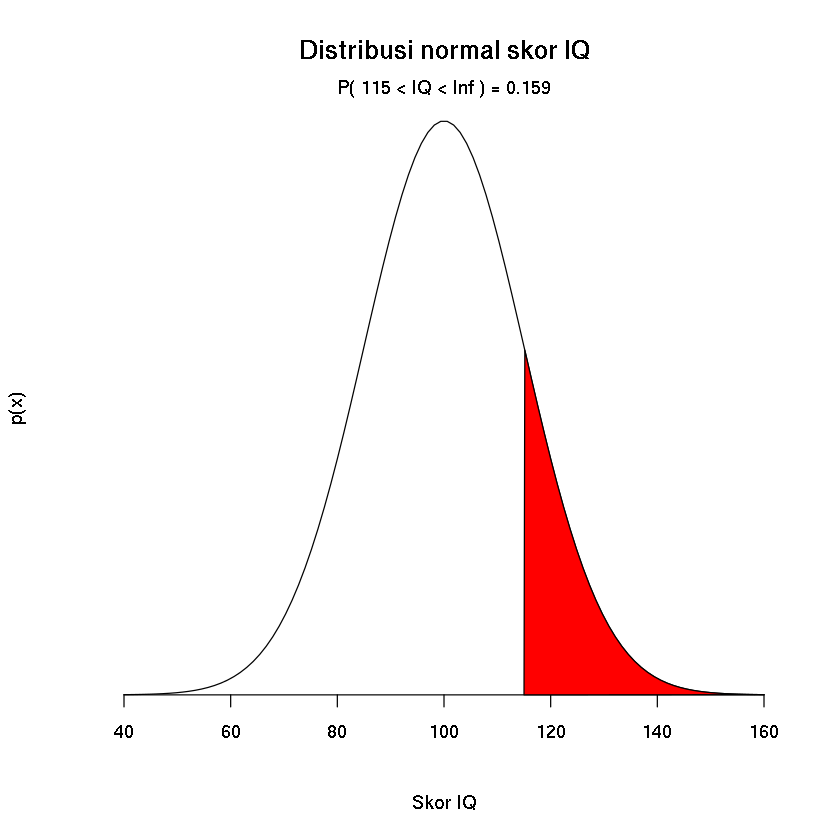
\includegraphics[width=0.9\textwidth]{gambar/gmb11.png}
    \caption{Distribusi normal IQ siswa.}
    \label{fig:fig11}
\end{figure}

\section{Laboratorium 5: Implementasi matriks kovarian di lingkungan R}
Kita akan membuat matriks kovarian di R dengan dua cara, yakni dengan membuat dari awal dan menggunakan fungsi bawaan (\textit{built-in}) dari R.

Mendefinisikan vektor kolom:


\begin{verbatim}
a <- 1:6
b <- seq(1, 11,by=2)
c <- seq(10, 60, by=10)
d <- c(2, 5, 5, 2, 1, 0)
e <- c(4, 5, 6, 7, 8, 9)        
\end{verbatim}



Membuat matriks dari vektor - vektor di atas:

\begin{verbatim}
M <- cbind(a,b,c,d,e)
k <- ncol(M)
n <- nrow(M)
print(M)        
\end{verbatim}

\begin{verbatim}
     a  b  c d e
[1,] 1  1 10 2 4
[2,] 2  3 20 5 5
[3,] 3  5 30 5 6
[4,] 4  7 40 2 7
[5,] 5  9 50 1 8
[6,] 6 11 60 0 9        
\end{verbatim}

Mencari rata - rata (ekspektasi) untuk setiap kolom:

\begin{verbatim}
k_rata2 <-  matrix(data = 1, nrow = n) %*% 
cbind(mean(a), mean(b), mean(c), mean(d), mean(e))
print(k_rata2)    
\end{verbatim}

\begin{verbatim}
     [,1] [,2] [,3] [,4] [,5]
[1,]  3.5    6   35  2.5  6.5
[2,]  3.5    6   35  2.5  6.5
[3,]  3.5    6   35  2.5  6.5
[4,]  3.5    6   35  2.5  6.5
[5,]  3.5    6   35  2.5  6.5
[6,]  3.5    6   35  2.5  6.5
\end{verbatim}


Mendefinisikan perbedaan antar matriks:

\begin{verbatim}
diffM <- M - k_rata2
print(diffM)
\end{verbatim}

\begin{verbatim}
        a  b   c    d    e
[1,] -2.5 -5 -25 -0.5 -2.5
[2,] -1.5 -3 -15  2.5 -1.5
[3,] -0.5 -1  -5  2.5 -0.5
[4,]  0.5  1   5 -0.5  0.5
[5,]  1.5  3  15 -1.5  1.5
[6,]  2.5  5  25 -2.5  2.5
\end{verbatim}

Mendefinisikan matriks kovarian:
\begin{verbatim}
Mkovar <- (n-1)^-1 * t(diffM) %*% 
diffM # kovarian sampel
print(Mkovar)
\end{verbatim}

\begin{verbatim}
     a  b   c     d    e
a  3.5  7  35  -2.5  3.5
b  7.0 14  70  -5.0  7.0
c 35.0 70 350 -25.0 35.0
d -2.5 -5 -25   4.3 -2.5
e  3.5  7  35  -2.5  3.5
\end{verbatim}

Mencari variansi dari matriks kovarian:
\begin{verbatim}
var <- diag(Mkovar)
print(var)
\end{verbatim}

\begin{verbatim}
    a     b     c     d     e 
  3.5  14.0 350.0   4.3   3.5 
\end{verbatim}

Kita dapat menggunakan fungsi \textit{built-in} \verb|cov()| untuk mendefinisikan matriks kovarian di lingkungan R:

\begin{verbatim}
print(cov(M))
\end{verbatim}

\begin{verbatim}
     a  b   c     d    e
a  3.5  7  35  -2.5  3.5
b  7.0 14  70  -5.0  7.0
c 35.0 70 350 -25.0 35.0
d -2.5 -5 -25   4.3 -2.5
e  3.5  7  35  -2.5  3.5
\end{verbatim}

\section{Distribusi - distribusi spesial}
Terdapat beberapa distribusi probabilitas yang umum dijumpai di hampir seluruh literatur tentang pemelajaran mesin, di antaranya adalah:
\subsection{Distribusi Bernoulli}
Merupakan suatu distribusi untuk peubah acak diskrit tunggal, dengan formulasi umum sebagai berikut:
\begin{equation}
    \begin{aligned}
        P(X=1) = \phi\\
        P(X=0) = 1 - \phi
    \end{aligned}    
\end{equation}
Distribusi ini dapat dikembangkan dengan melibatkan banyak peubah acak menjadi distribusi multinomial.

\subsection{Distribusi multinomial}
Distribusi yang melibatkan banyak peubah acak diskrit yang mana merupakan pengembangan dari distribusi Bernoulli. Kedua distribusi ini dapat dikatakan bisa memodelkan hampir seluruh distribusi probabilitas diskrit.

\subsection{Distribusi Gaussian}
Distribusi Gaussian (Gambar \ref{fig:fig12}) juga dikenal sebagai distribusi normal. Distribusi ini merupakan distribusi untuk peubah acak kontinyu yang dapat memodelkan hampir 90\% permasalahan statistik yang melibatkan bilangan riil. Oleh karenanya distribusi ini merupakan bagian integral dari hampir seluruh algoritma pemelajaran mesin yang melibatkan peubah acak kontinyu. Formulasi umum dari distribusi ini ditampilkan pada persamaan \ref{eqn:eqn49}:

\begin{equation}
    \mathcal{N}(x;\,\mu,\,\sigma^{2}) = \sqrt{\frac{1}{2\pi \sigma^2}} \exp{\left(-\frac{1}{2\sigma^2} (x-\mu)^2\right)}
    \label{eqn:eqn49}
\end{equation}

\begin{figure}[H]
    \centering
    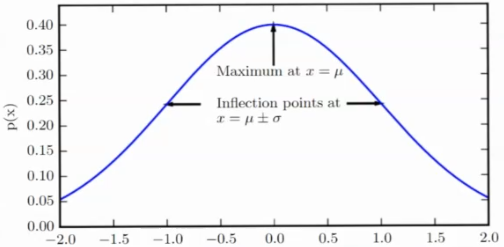
\includegraphics[width=0.9\textwidth]{gambar/gmb12.png}
    \caption{Distribusi normal.}
    \label{fig:fig12}
\end{figure}

Terdapat tiga buah aturan penting terkait sebaran data di dalam distribusi Gaussian, di antaranya adalah:
\begin{itemize}
    \item 68\% data tersebar di dalam jangkauan $\mu \pm{} \sigma$.
    \item 95\% data tersebar di dalam jangkauan $\mu \pm{} 2\sigma$.
    \item 99,7\% data tersebar di dalam jangkauan $\mu \pm{} 3\sigma$.
\end{itemize}

\subsection{Distribusi eksponensial}
Merupakan distribusi probabilitas kontinyu dengan titik lancip pada $x = 0$. Formulasi umumnya ditunjukkan pada persamaan \ref{eqn:eqn50} berikut ini:
\begin{equation}
    p(x;\,\lambda) = \lambda1_{x \geq 0} \exp{(-\lambda x)}
    \label{eqn:eqn50}
\end{equation}

\subsection{Distribusi Laplace}
Distribusi probabilitas dengan titik tajam pada $x = \mu$. $\mu$ di sini tidak harus berupa nilai rata - rata, melainkan titik sebarang tempat tempat titik lancip berada. Formulasi umumnya ditunjukkan pada persamaan \ref{eqn:eqn51} berikut ini:
\begin{equation}
      \text{Laplace}(x;\,\mu,\, \gamma) = \frac{1}{2\gamma}\exp{\left(\frac{-|x - \mu|}{\gamma}\right)}
      \label{eqn:eqn51}
\end{equation}


\blankpage
\chapter{Latihan Pemantapan Konsep}
\section{Soal}
\begin{enumerate}
    \item Dengan menggunakan NumPy hitunglah jumlah baris dan kolom pada matriks - matriks berikut ini:
        \begin{enumerate}[label=(\Alph*)]
            \item $\begin{bmatrix} 1 & 0 & 0\\0 & 1 & 0\\0 & 0 & 1 \end{bmatrix}$
            \item $\begin{bmatrix}2 & 1 & 1\\ 1 & 2 & 8\end{bmatrix}$
            \item $\begin{bmatrix}1 & -1 & 1\end{bmatrix}$
            \item $\begin{bmatrix}1 & 2 \\ 8 & 1\end{bmatrix}$
            \item $\begin{bmatrix} 1 & 0 \\ 0 & 1\\ 0 & 0\\ 2 & 1 \end{bmatrix}$
            \item $\begin{bmatrix}2 & 1 & 1 & 2\\ 1 & 2 & 2 & 1 \end{bmatrix}$
        \end{enumerate}
    \item Dengan menggunakan NumPy, hitunglah transpos pada matriks - matriks berikut ini:
        \begin{enumerate}[label=(\Alph*)]
            \item $\begin{bmatrix}6 & 5 & 4 & 2\\1 & 5 & 2 & 1\\ 7 & 0 & 2 & 1\\ 1 & 2 & 3 & 4\end{bmatrix}$
            \item $\begin{bmatrix}2 & 1 & 1\\ 1 & 3 & 2\end{bmatrix}$
        \end{enumerate}
    \item Dengan menggunakan NumPy, hitunglah norma $L^2$ dari vektor $\mathbf{x}$ sebagai berikut:
    $\mathbf{x} = \begin{bmatrix}1 & 2 & 3 & 4\end{bmatrix}$
    \item Carilah turunan pertama dari:
    \begin{enumerate}[label=(\Alph*)]
        \item $f(x,y) = x^{4}y + 2x$
        \item $f(x,y) = 2y + 3x^{2}$
    \end{enumerate}
    \item \textbf{Pilihlah jawaban yang paling tepat!}
    
    Arah penurunan dari fungsi objektif $f(x)$ dapat diketahui melalui:
    \begin{enumerate}[label=(\Alph*)]
        \item Gradien $(\nabla)$
        \item Gradien negatif $(-\nabla)$
        \item Matriks Jacobian $(\mathbf{J})$
        \item Laplacian $(\nabla^2)$
    \end{enumerate}
    
    \item \textbf{Lengkapi bagian kosong pada soal sebagai berikut: }
    
    Integral \underline{\hspace{3cm}} dari $f(x)$ merupakan bilangan representasi dari wilayah di bawah kurva dari $x = a$ hingga $x = b$. Integral \underline{\hspace{3cm}} dari $f(x)$ tidak mempunyai batas dan hasil akhirnya berupa suatu fungsi.
    
    \item \textbf{Lengkapi bagian kosong pada soal sebagai berikut: }
    
    Titik kritis dari suatu fungsi konveks sudah pasti merupakan titik minimum \underline{\hspace{3cm}}.
    
    \item Carilah titik minimum global dari fungsi objektif $f(x) = 2x^{2} - 3$!
    \item \textbf{Lengkapi bagian kosong pada soal sebagai berikut: }
    
    \underline{\hspace{3cm}} merupakan sumber dari sifat stokastik yang melekat pada sistem yang dimodelkan, pemodelan yang tidak tepat, dan tidak nya data pengamatan.
    
    \item \textbf{Lengkapi bagian kosong pada soal sebagai berikut: }
    
    Distribusi probabilitas untuk peubah acak kontinyu dinamakan sebagai \underline{\hspace{3cm}}.
    
    \item \textbf{Lengkapi bagian kosong pada soal sebagai berikut: }
    
    Simbol matematis untuk rata - rata, varian, dan standar deviasi adalah: \underline{\hspace{1cm}}, \underline{\hspace{1cm}}, \underline{\hspace{1cm}}.
    
    \item Tuliskanlah persamaan yang digunakan untuk memodelkan ekspektasi pada peubah acak diskrit!
    
    \item \textbf{Lengkapi bagian kosong pada soal sebagai berikut: }
    
    Distribusi probabilitas yang umum dijumpai di alam adalah distribusi \underline{\hspace{3cm}}.
\end{enumerate}

\section{Jawaban}
\begin{enumerate}
\item\\
\lstinputlisting[language=Python]{jwb1.py}
Hasilnya:
\begin{verbatim}
Jumlah baris A: 3, Jumlah kolom A: 3.
Jumlah baris B: 2, Jumlah kolom B: 3.
Jumlah baris C: 3, Jumlah kolom C: 3.
Jumlah baris D: 2, Jumlah kolom D: 2.
Jumlah baris E: 4, Jumlah kolom E: 2.
Jumlah baris F: 2, Jumlah kolom F: 4.
\end{verbatim}

\item\\
\lstinputlisting[language=Python]{jwb2.py}
Hasilnya:
\begin{verbatim}
[[6 1 7 1]
 [5 5 0 2]
 [4 2 2 3]
 [2 1 1 4]]
################
[[2 1]
 [1 3]
 [1 2]]
\end{verbatim}

\item\\
\lstinputlisting[language=Python]{jwb3.py}
Hasilnya:
\begin{verbatim}
Norma Euklidesan dari vektor x adalah: 5.477225575051661
\end{verbatim}

\item 
\begin{enumerate}[label=(\Alph*)]
    \item $\nabla f(x,y) = \left[4x^{3} + 2,\, x^{4}\right]$
    \item $\nabla f(x,y) = \left[6x,\, 2\right]$
\end{enumerate}

\item \textbf{B}. Gradien negatif $(-\nabla)$

\item Integral \textbf{tentu} dari $f(x)$ merupakan bilangan representasi dari wilayah di bawah kurva dari $x = a$ hingga $x = b$. Integral \textbf{tak-tentu} dari $f(x)$ tidak mempunyai batas dan hasil akhirnya berupa suatu fungsi.

\item Titik kritis dari suatu fungsi konveks sudah pasti merupakan titik minimum \textbf{global}. 
\item 
$f(x) = 2x^{3} -3$\\\\
$\frac{df(x)}{dx} = 2(2)x - 4x$\\
\begin{itemize}
\item Turunan pertama dinyatakan dalam bentuk nol:\\
$0 = 4x$\\
$x = 0$ (merupakan titik kritis)
\item Uji coba turunan kedua:\\\\
$\frac{d^{2}f(x)}{dx} = 4$\\\\
Karena turunan kedua bernilai positif dan tidak ada titik - titik kritis lainnya, maka $x=0$ dinyatakan sebagai titik minimum global.
\end{itemize}
\item \textbf{Ketidakpastian} merupakan sumber dari sifat stokastik yang melekat pada sistem yang dimodelkan, pemodelan yang tidak tepat, dan tidak nya data pengamatan.
\item Distribusi probabilitas untuk peubah acak kontinyu dinamakan sebagai \textbf{fungsi kepadatan peluang} (\textbf{probability density function}).
\item Simbol matematis untuk rata - rata, varian, dan standar deviasi adalah: $\mu$, $\sigma^2$, dan $\sigma$.
\item $	E_{x \sim\ p}\left[f(x)\right] = \sum_{x} P(x)f(x)$
\item Distribusi probabilitas yang umum dijumpai di alam adalah distribusi \textbf{Gaussian (normal)}.
\end{enumerate}
\blankpage

\nocite{*}
\bibliographystyle{unsrt}
\bibliography{pustaka}
\end{document}